\clearpage
\thispagestyle{empty}
\null
\newpage

\cleardoublepage
\phantomsection
% \pdfbookmark[1]{State of the art}{State of the art}
% \addcontentsline{toc}{part}{State of the art}
\markboth{\spacedlowsmallcaps{State of the art}}{\spacedlowsmallcaps{State of the art}}
\part{State of the art}
\label{part:state_art}

\clearpage
\thispagestyle{empty}
\null
\newpage

% \acn{TODO}:
% - Overall, harmonize the vocabulary
% - Overall, correctly introduce technical/theoretical terms such as “Organizational Adequacy,” “\acn{RNN},” “\acn{VAE},” “\acn{LSTM},” “World Models,” in particular to enable readers unfamiliar with \acn{ML} or \acn{AI} in general to understand.
% - Reformat to highlight the sub-problem accompanied by the associated hypothesis, then establish the state of the art in the research space defined by the hypothesis in order to address the sub-problem: provide an overview of the state of the art with a summary in table form that shows how the work (belonging to this research space delimited by the hypothesis) best addresses the sub-problems (i.e., how a piece of work covers the objectives of a sub-problem). This also allows us to see which objectives of the sub-problems are well covered in the literature, moderately covered, or not covered at all. So in the end, we can determine which work covers the most objectives of a sub-problem, but also which objectives are still not covered, presented in the form of theoretical or technical barriers.
% - In the end, we should therefore know which works are the most promising and which barriers remain to be overcome by contributions that will be presented in the next section on the method.

\chapter*{Introduction}
\addcontentsline{toc}{chapter}{\textbf {Introduction}}

\noindent
This section aims to identify and analyze the most relevant approaches to solving the four sub-problems resulting from the decomposition of the problem of designing a Cyberdefense \acn{SMA}, formalized as a constrained optimization problem. The objective is to identify the work that meets the specific criteria of each sub-problem, while highlighting the scientific and technical obstacles that remain, in order to capitalize on existing advances.

The first chapter provides a critical review of the literature for each of the sub-problems, based on the four main activities of the approach. For each activity, the aim is to identify the major contributions likely to meet the criteria set, as well as the main obstacles that justify the need for new methodological advances.

The second chapter takes a closer look at the work identified as most promising, in order to provide a solid theoretical foundation for explaining and technically defining the obstacles identified. This chapter thus introduces the fundamental concepts that will serve as the basis for future methodological contributions to the proposed method.

\autoref{fig:manuscript_organization_part_2} summarizes the organization of this part and the logical links between chapters and subsections.


\begin{figure}[h!]
  \centering
  \resizebox{0.8\textwidth}{!}{%
    \input{figures/manuscript_organization_part_2}
  }
  \caption{Structure of Part II: State of the art}
  \label{fig:manuscript_organization_part_2}
\end{figure}

\clearpage
\thispagestyle{empty}
\null
\newpage


\chapter{Barriers to a design method}
\label{chap:barriers}

\noindent
The purpose of this chapter is to introduce and analyze the main scientific barriers related to the automated design of \acplu{SMA}, as they emerge from the breakdown of the problem into four main activities: modeling, resolution, analysis, and transfer. For each of these activities, a fundamental sub-problem (\textbf{MOD} to \textbf{TRF}) has been identified, associated with a hypothesis restricting the search space (\textbf{H-MOD} to \textbf{H-TRF}) . For each sub-problem, we define a set of specific criteria for evaluating the coverage of existing approaches. The literature review conducted according to these criteria allows us to map the most relevant work, identify major advances, and highlight remaining obstacles and gaps. This chapter thus offers a critical analysis of the state of the art for each hypothesis, with a view to identifying the challenges to be addressed and motivating the methodological contributions presented in the rest of the manuscript.

\section{Modeling an environment in simulation (H-MOD)}

\subsection*{Recontextualization of the sub-problem in the thesis approach}

The first fundamental sub-problem identified in our approach concerns the \textbf{realistic modeling of the environment} (\textbf{MOD}) . This step is crucial because it determines the credibility of the experiments, the training of the agents, and, ultimately, the validity of the cyberdefense policies obtained. In the context of the thesis, simulating a relevant environment makes it possible to test, evaluate, and optimize multi-agent behaviors without exposing real systems to operational risks. It thus constitutes the experimental foundation on which the subsequent phases of learning, analysis, and transfer are based. \subsection* {Overall objective and specific criteria} The main objective of this activity is to obtain a simulated environment that is \textbf{realistic}, \textbf{adaptable}, \textbf{faithful to real-world dynamics}, and \textbf{usable for training and evaluating agents}. To guide the literature review, we have selected the following specific criteria:
%
\begin{itemize}
  \item \textbf{Fidelity}: ability to reproduce the dynamics, threats, and interactions observed in real environments; \emph{this criterion is essential to ensure that the policies learned in simulation are relevant and transferable to the real world}.
  \item \textbf{Adaptability}: ability to easily modify the topology, scenarios, or parameters to explore different contexts; \emph{this allows testing the robustness of agents in various environments and studying multiple use cases}.
  \item \textbf{Automation}: degree of automation in the generation or evolution of the simulated environment; \emph{a high degree of automation facilitates the rapid creation of new scenarios and reduces dependence on human expertise}.
  \item \textbf{Interoperability}: ability to integrate or exchange data with other tools or platforms; \emph {this criterion promotes the reuse, comparison, and integration of results from different systems or data sources}.
  \item \textbf{Ease of use}: accessibility for designers, possibility of customization without advanced expertise; \emph{ease of use speeds up prototyping and democratizes experimentation among non-specialist users}.
  \item \textbf{Multi-agent}: ability of the environment to accommodate one or more agents and manage their interactions; \emph{this criterion is essential for studying collaborative or competitive scenarios and for evaluating multi-agent approaches}.
\end{itemize}

\subsection*{Research space restriction hypothesis (\textbf{H-MOD})}

In order to limit the research space to a relevant and exploitable domain, we make the following assumption: \textit{It is possible to obtain a realistic simulated environment, either by facilitating manual modeling or by using machine learning techniques based on data} . This hypothesis leads us to focus our literature review on two main families of work:

\begin{itemize}
  \item \textbf{Manual modeling}: includes all work in which the creation of the simulated environment relies on human intervention. This includes simulators (\acn{CybORG}, \acn{NASimEmu}, \acn{CYST}) and generic cyberdefense environment models, in which the structure, rules, and scenarios are explicitly defined, either fully or partially, by experts. This approach allows existing models to be reused, either directly if the simulated environment corresponds to the real target environment, or after adaptation and instantiation of the generic simulation model. Although widely used, this method often limits genericity, as few models are both easy to adapt and applicable to a wide variety of cyber defense environments. It also includes Markovian formalisms (\acn{MDP}, \acn{POMDP}, \acn{Dec-POMDP}, \acn{POSG}), which serve as the theoretical and practical basis for most manual modeling.
  \item \textbf{Learning-based modeling}~: includes approaches where the dynamics of the environment are learned automatically from data collected in the real environment or from interactions. This includes work on system identification, surrogate modeling, and data-driven simulation.
\end{itemize}

This choice is motivated by the state of the art, which shows that these two areas account for most of the recent advances and offer different trade-offs between fidelity, automation, and adaptability.

\subsection*{Coverage of criteria by the identified work}

A summary of the coverage of the criteria by the work identified in the topics mentioned in the hypothesis (\textbf{H-MOD}) is presented in \autoref{tab:couverture_criteres_travaux}.

\begin{table}[h!]
  \centering
  \caption{Coverage of specific criteria by the main families of cyberdefense environment modeling work}
  \label{tab:couverture_criteres_travaux}
  \tiny
  \renewcommand{\arraystretch}{1.4}
  \begin{tabularx}{\textwidth}{
      >{\raggedright\arraybackslash\hsize=0.4\hsize}X
      >{\raggedright\arraybackslash\hsize=0.1\hsize}X
      >{\raggedright\arraybackslash\hsize=0.1\hsize}X
      >{\raggedright\arraybackslash\hsize=0.1\hsize}X
      >{\raggedright\arraybackslash\hsize=0.1\hsize}X
      >{\raggedright\arraybackslash\hsize=0.1\hsize}X
      >{\raggedright\arraybackslash\hsize=0.1\hsize}X
    }
    \hline
    \textbf{Work / Criteria}                                                                                                            & \textbf{Fidelity} & \textbf{Adaptability} & \textbf{Automation} & \textbf{Interoperability} & \textbf{Ease of use} & \textbf{Multi-agent} \\
    \hline
    Generic formal models (\acn{MDP}, \acn{POMDP}, \acn{Dec-POMDP}, \acn{POSG}, attack graphs, \acn{AD} trees, Petri nets, game models) & \cmark{}          & \cmark{}              & \xmark{}            & \cmark{}                  & \xmark{}             & \cmark{}             \\
    Generic and configurable frameworks (\acn{CyberBattleSim}, \acn{NASim}, \acn{NASimEmu}, \acn{DETERLab}, \acn{CyberVAN}, \acn{CYST}) & \cmark{}          & \cmark{}              & \xmark{}            & \cmark{}                  & \cmark{}             & \cmark{}             \\
    Specialized cyber defense simulators (\acn{CybORG}, \acn{CybORG}++, CyberWheel, \acn{SCYTHE}, \acn{CTF})                            & \cmark{}          & \xmark{}              & \xmark{}            & \cmark{}                  & \cmark{}             & \cmark{}             \\
    System Identification                                                                                                               & \cmark {}         & \cmark{}              & \cmark{}            & \xmark{}                  & \xmark{}             & \cmark{}             \\
    Surrogate Modeling                                                                                                                  & \cmark{}          & \cmark{}              & \cmark{}            & \xmark{}                  & \cmark{}             & \cmark{}             \\
    Data-Driven Simulation (World Models)                                                                                               & \cmark{}          & \cmark{}              & \cmark{}            & \xmark{}                  & \xmark{}             & \cmark{}             \\
    \hline
  \end{tabularx}
\end{table}

Regarding the manual modeling approach, the identified works are:

\paragraph{Generic formal models.}
At the most abstract level, the modeling of cyberdefense environments is based on mathematical formalisms derived from sequential decision theory. The basic framework is the \textit{Markov Decision Process} (\acn{MDP})~\cite{puterman1994mdp}, which describes an environment as a set of states, actions, and probabilistic transitions. When the available information is partial, \acn{POMDP}~\cite{kaelbling1998pomdp} offer a suitable framework. For cooperative \acplu{SMA}, decentralized variants (\acn{Dec-POMDP})~\cite{Oliehoek2016} are used, while competitive (attacker/defender) environments are modeled by \textit{Partially Observable Stochastic Games} (\acn{POSG})~\cite{hansen2004posg}. Other extensions, such as factorized \acn{MDP}~\cite{guestrin2003factored}, facilitate the modeling of complex systems, and security game theory~\cite{manshaei2013game} allows adversarial strategies to be explicitly formalized.
These formalisms form the common theoretical basis for most cybersecurity simulators and frameworks. Alongside Markovian models, intermediate graphical representations are also used. Attack graphs~\cite{CPhilips1998} describe the different ways in which a network's vulnerabilities can be exploited, while attack-defense trees~\cite{BKordy2010} explicitly incorporate defensive countermeasures. Petri nets ~\cite{MPetty2022,JBland2020,SYamaguchi2020} can be used to represent and analyze competing attack and defense strategies. Finally, game models applied to cybersecurity~\cite{MPanfili2018,AAttiah2018,CXiaolin2008} formalize attacker/defender interactions as dynamic, often non-cooperative games, and provide a natural bridge to the \acn{POSG} and \acn{Dec-POMDP} frameworks~\cite{beynier2010,terry2020pettingzoo,bernstein2013}.
In summary, these formal and graphical models offer a generic and flexible toolkit for building simulation environments suitable for a wide variety of cybersecurity scenarios.

\paragraph{Generic and configurable frameworks.}
Between abstract formalisms and specialized simulators, the literature highlights several frameworks that aim to offer a compromise between generality and usability. Among these, \acn{CyberBattleSim}~\cite{cyberbattlesim}, developed by Microsoft, offers configurable modeling of a network in the form of a graph, where each node represents a vulnerable service. Similarly, \textit{NASim}~\cite{nasim2023} and its extension \acn{NASimEmu}~\cite{fernandes2024nasimemu} allow the definition of various topologies, vulnerabilities, and attack scenarios, with compatibility with OpenAI Gym facilitating use in reinforcement learning. Other approaches are found in large-scale test infrastructures such as \textit{DETERLab} and \textit{CyberVAN}~\cite{Mirkovic2010}, which offer configurable environments for cyber simulation and emulation. In addition, the \textit{CYST}~\cite{Drasar2020} tool offers a modular platform for creating and evaluating cyber defense scenarios, with an emphasis on flexibility and extensibility. These frameworks are distinguished by their ability to be adapted to different contexts, while providing environments that are sufficiently realistic for training and evaluating cyber defense agents.

\paragraph {Specialized cyber defense simulators.}
Finally, at the most concrete level, several dedicated simulators have been developed to provide instantiated environments in which cyber defense agents can be trained and evaluated. Among them, \acn{CybORG}~\cite{Standen2021} has become a benchmark, with Red Team/ Blue Team scenarios that can be used in competitions such as the \acn{CAGE} Challenge, and which has been extended in \acn{CybORG}++ to integrate \acn{Dec-POMDP} models and complex multi-agent scenarios~\cite {landolt2025cyborgpp}. The \textit{CyberWheel}~\cite{vyas2025cyberwheel} simulator has also been proposed for the academic training of automated defenders, with an emphasis on education. In addition to these research tools, \textit{capture-the-flag} oriented platforms such as \textit{SCYTHE} or \acn{CTF}~\cite{palmer2023ctf} environments have been repurposed to serve as test beds for reinforcement learning approaches in cyber defense. These specialized simulators are distinguished by their high degree of fidelity and their focus on specific use cases, but at the cost of more limited adaptability compared to generic frameworks.

\

Regarding the automatic modeling approach, the identified works are:

\paragraph{System Identification.}
A first family of works automates the construction of simulated environments via system identification methods, where real-world dynamics are reconstructed from empirical data. These approaches seek to automatically extract equations or models describing the evolution of a system, for example in microgrid or \acplu{SMA} contexts subject to attacks~\cite{NtDvjag65BgJ, tBI-_piWs1cJ} . Identification can be performed through parametric or structural estimation of control models~\cite{g5PxHs45ZtYJ}, but also by adjusting probabilistic/stochastic models that directly incorporate dynamic uncertainty and are calibrated using real data. These probabilistic models include Bayesian Markov processes, dynamic Bayesian networks, and Gaussian processes, which can capture nonlinear and uncertain behavior in complex environments. Such work illustrates how system identification provides an automated and statistically robust basis for simulating cyberdefense environments from traces and measurements.

\paragraph{Surrogate Modeling.}
A second family includes work on \textit {surrogate modeling}, where an approximate, lightweight model is trained to reproduce the behavior of a simulator or costly system. These models are particularly useful in cyber-physical environments where running a high-fidelity simulator is too burdensome to allow for mass training of agents. This includes approaches using neural networks or graph neural networks as surrogate models~\cite{g4qXIBHVJwUJ, Cr1JpifjcFwJ}, as well as probabilistic methods for estimating the distribution of system outputs~\cite{hPBZHSLGStkJ} . These surrogate models can be distributed and integrated into federated architectures to preserve data confidentiality while improving the speed and performance of simulations~\cite{g4qXIBHVJwUJ}. They offer an effective compromise between realism and exploitability, providing agents with environments that are close to reality but more accessible computationally.

\paragraph{Data-Driven Simulation.}
Finally, the third family is based on simulation approaches directly guided by data collected in real environments. These approaches construct a partial or complete digital twin of the target system using observed traces, logs, and trajectories. An emblematic example is that of \textit{World Models}~\cite{Ha2018}, which use neural architectures to learn a compact latent space that allows the dynamics of an environment to be simulated and generalized based on past interactions. In the context of cybersecurity, these models can simulate the behavior of attackers and defenders by directly exploiting network logs or data from past incidents~\cite{D2mbiT0vgP4J} . More broadly, data-driven simulation approaches combine deep learning, symbolic representations, and multi-agent reinforcement learning~\cite{5oUSbVbTXX0J, RQyw5NYMj-wJ} to create artificial but realistic environments capable of capturing the co-evolution of attack and defense~\cite{oOfK6FXUSCAJ}. This work paves the way for simulated environments whose fidelity and adaptability increase with the richness of the data collected.

\subsection* {Analysis of work and obstacles}

Analysis of manual modeling work shows that generic formal models, in particular the \acn{Dec-POMDP} framework, offer the best adaptability and generality for representing multi-agent cyberdefense environments. Unlike configurable frameworks or specialized simulators, which are often limited by their internal structure and difficulty in adapting to new contexts, a \acn{Dec-POMDP} model allows any scenario to be formalized using standardized abstractions (states, actions, observations, rewards). However, this flexibility comes at a cost: manually modeling a realistic environment remains a cumbersome task, requiring advanced expertise and a significant formalization effort. Furthermore, automation of this step is very limited, as there is no library of pre-specialized \acn{Dec-POMDP} models for cybersecurity that would factor in the invariants common to these environments. Thus, even though \acn{Dec-POMDP} is the most relevant choice for ensuring adaptability, it does not meet the automation criterion and imposes a high barrier to entry for modeling new environments.

On the automatic modeling side, system identification and surrogate modeling approaches offer interesting solutions for automating model generation from data, but they often require mathematical pre-modeling or fine calibration on specific datasets. World Models stand out as the most promising solution for automating modeling, as they directly learn the observational dynamics of the environment without requiring any explicit prior structure. This approach offers high fidelity and great agility, regardless of the domain of application. However, one obstacle remains: current World Models are mainly designed for single-agent contexts, and their extension to multi-agent contexts remains an open challenge, particularly when it comes to capturing complex interactions between agents. Furthermore, full automation is hampered by the need to tune hyperparameters and adapt the model architecture to each new use case. In summary, while World Models represent the most automated and accurate option, they do not yet fully cover the needs of a multi-agent cyberdefense environment without human intervention.

\section{The integration of constraints in MARL (H-TRN)}

\subsection*{Recontextualization of the sub-problem in the thesis approach}

The second fundamental sub-problem in our approach concerns the \textbf{ability to integrate explicit organizational constraints or guidance into the multi-agent learning process} (\acn{MARL}). While \acn {MARL} allows agents to autonomously discover cooperative policies in complex environments, it does not, as it stands, guarantee compliance with essential organizational specifications such as role distribution, structured coordination, or compliance with safety rules.

In the context of cyber defense, this issue is particularly important. Environments are not only dynamic and partially observable, but they also impose stringent requirements in terms of security, robustness, and explainability. It is not enough for agents to learn to cooperate effectively: it is often essential that they respect predefined organizational constraints, for example to ensure the separation of responsibilities, the hierarchy of decisions, or compliance with defense protocols.

This sub-problem is therefore central to the thesis, which aims to reconcile the learning autonomy offered by \acn{MARL} with the need to guarantee critical organizational properties. The integration of such organizational constraints or guidance into the learning process should ensure the consistency, safety, and explainability of collective behaviors, while preserving the agents' ability to adapt to evolving threats. This issue thus structures one of the major axes of the proposed method, seeking to overcome the limitations of purely emergent or purely prescriptive approaches in the design of \acplu{SMA} for cyber defense.

To evaluate the ability of existing approaches to integrate organizational constraints or guidance into the multi-agent learning process, we use the following specific criteria:
\begin{itemize}
  \item \textbf{Expressiveness of constraints}: ability to express complex organizational requirements (roles, missions, interactions, hierarchies);
        \emph{this criterion is essential to ensure that relevant organizational constraints in the domain can be formalized and taken into account in learning.}
  \item \textbf{Level of integration}~: level at which constraints are taken into account (action, policy, trajectory, organization); \emph{this criterion allows the granularity and scope of constraints to be assessed, as well as their impact on the collective behavior of agents.}
  \item \textbf{Guarantee of compliance}~: existence of theoretical or empirical guarantees that constraints will be satisfied; \emph{this criterion is essential to ensure that critical organizational properties are not violated when learned policies are executed.}
  \item \textbf{Compatibility with learning}: maintenance of the agents' ability to adapt and optimize; \emph{this criterion aims to ensure that the integration of constraints does not hinder the flexibility and effectiveness of multi-agent learning.}
  \item \textbf{Explainability}: ability to explain or verify compliance with constraints in learned policies; \emph{this criterion is fundamental to enable the analysis, validation, and certification of collective behaviors with respect to organizational requirements.}
\end{itemize}

\subsection*{Search space restriction hypothesis (\textbf{H-TRN})}

In order to limit the search space to a relevant and exploitable domain, we adopt the following hypothesis:

\textit{It is possible to integrate explicit organizational constraints or guidance into the multi-agent learning process in order to guide or restrict the space of learned policies, while preserving the agents' ability to adapt and optimize.}

This hypothesis leads us to explore three main complementary areas in the literature:
\begin{itemize}
  \item \textbf{The integration of explicit constraints}: work in which safety, structural, or mission constraints are formally added to the learning process (e.g., via Constrained \acn{MDP}, \acn{CPO}, Deep Constrained Q-Learning, etc.) ;
  \item \textbf{The use of guidance mechanisms}: approaches that guide learning through techniques such as reward shaping, shielding, or the incorporation of human feedback, in order to indirectly influence the learned policies;
  \item \textbf{Incorporating symbolic organizational models}~: attempts to integrate organizational specifications from \acn{SMA} engineering (mainly \acn{AGR}~\cite{Ferber2004} and $\mathcal{M} OISE^+$~\cite{hubner2002moise}) into the learning process in order to ensure compliance with structures, roles, or collective missions.
\end{itemize}

The scope of the literature review is thus delimited by these three axes, which cover all approaches aimed at combining multi-agent learning and compliance with organizational constraints, whether explicitly, implicitly, or symbolically imposed.

\subsection*{Coverage of criteria by the identified works}

A summary of the coverage of these criteria by the main families of works identified is presented in \autoref{tab:couverture_criteres_travaux_trn}.

\begin{table}[h!]
  \centering
  \caption{Coverage of criteria by the main families of work on the integration of organizational constraints/guidance in MARL}
  \label{tab:couverture_criteres_travaux_trn}
  \scriptsize
  \renewcommand{\arraystretch}{1.4}
  \begin{tabularx}{\textwidth}{
    >{\raggedright\arraybackslash\hsize=0.25\hsize}X
    >{\raggedright\arraybackslash\hsize=0.15\hsize}X
    >{\raggedright\arraybackslash\hsize=0.15\hsize}X@{\hspace{1cm}}
    >{\raggedright\arraybackslash\hsize=0.15\hsize}X
    >{\raggedright\arraybackslash\hsize=0.15\hsize}X
    >{\raggedright\arraybackslash\hsize=0.15\hsize}X
    }
    \hline
    \textbf{Work / Criteria}                                                                                                                                                                     & \textbf{Organizational expressiveness} & \textbf{Level of integration} & \textbf{Guarantee of compliance} & \textbf{Learning compatibility} & \textbf{Explainability} \\
    \hline
    Safe \acn{RL}~\cite{garcia2015comprehensive}, \acn{CPO}~\cite{achiam2017constrained}, Deep Constrained Q-Learning~\cite{kalweit2020deep}                                                     & Low                                    & Action/Policy                 & Yes (partial)                    & Yes                             & Low                     \\
    Reward shaping~\cite{ng1999policy}, shielding~\cite{amodei2016concrete}, human feedback~\cite{warnell2018deep,zhou2025mentor}                                                                & Medium                                 & Action/Trajectory             & No (flexible)                    & Yes                             & Low                     \\
    Constraint-Guided \acn{RL}~\cite{spieker2021constraint}, \acn{MENTOR}~\cite{zhou2025mentor}, constrained \acn{RL} without explicit reward~\cite{miryoosefi2022}                              & Medium                                 & Policy                        & Yes (partial)                    & Yes                             & Medium                  \\
    Integration of organizational models ($\mathcal{M}OISE^+$~\cite{hubner2007using}, \acn{AGR}~\cite{Ferber2004}), learning/organization hybridization~\cite{bordini2006jade,chernova2014robot} & Strong (potential)                     & Organization                  & No (lock)                        & No (lock)                       & Strong                  \\
    \hline
  \end{tabularx}
\end{table}

The \autoref{tab:couverture_critères_travaux_trn} summarizes the work identified in the three areas defined by the hypothesis (\textbf{H-TRN}) with regard to specific criteria.

First, approaches from the field of Safe Reinforcement Learning, such as \acn{CPO}~\cite{achiam2017constrained} or Deep Constrained Q-Learning~\cite{kalweit2020deep}, are distinguished by their ability to provide certain guarantees of safety or partial compliance with constraints~\cite {garcia2015comprehensive}. This work generally operates at a local level, often at the level of actions or policies, and is well compatible with deep learning algorithms. However, their organizational expressiveness remains weak, as they do not explicitly model collective structures or organizational rules. Similarly, their explainability remains limited, making it difficult to interpret multi-agent behaviors in relation to organizational expectations. In short, these approaches favor local operational efficiency over overall consistency with complex organizational constraints.

Next, methods such as reward shaping~\cite{ng1999policy}, shielding~\cite{amodei2016concrete}, {ng1999policy}, shielding~\cite{amodei2016concrete}, or the integration of human feedback~\cite{warnell2018deep, zhou2025mentor} seek to influence agents through flexible or indirect mechanisms. Although these approaches allow for integration at different levels (actions or trajectories) and are compatible with learning, they do not offer formal guarantees regarding compliance with organizational constraints. Their expressiveness is relatively average, in that they can encode preferences, but without an explicit hierarchical structure. Furthermore, explainability is often low, as the source of certain decisions or adaptations by agents is diluted in the learning dynamics and implicit optimization of modified rewards. These methods are therefore useful for influencing agent behavior without imposing a rigid structure, but they struggle to bring about explicit organizational coordination.

More recent work on integrating constraints into multi-agent learning includes approaches such as Constraint-Guided \acn{RL}~\cite{spieker2021constraint}, \acn{MENTOR}~\cite{zhou2025mentor}, and constrained learning without an explicit reward function~\ cite{miryoosefi2022}. These methods aim to integrate explicit constraints or hierarchical guidance into the learning process, thus offering better compatibility with organizational requirements, although coverage remains partial. They represent a step towards a more systematic consideration of constraints in \acn{MARL}, while maintaining the adaptability of agents.

Finally, approaches based on the integration of explicit organizational models offer strong organizational expressiveness, as they allow for the formal representation of roles, missions, and relationships between collective entities. Among existing models, $\mathcal{M}OISE^+$ stands out as the most advanced and widely used in the SMA community, surpassing in particular \acn{AGR}~\cite{Ferber2004}. It allows for the integrated modeling of structural, functional, and deontic specifications, which facilitates the expression of complex organizational constraints and their compatibility with learning approaches.
%
However, a major technical obstacle remains: the direct integration of $\mathcal{M}OISE^+$ with learning methods is still very limited, if not non-existent, which means that effective compliance with organizational constraints during learning cannot be guaranteed. On the other hand, this model stands out for its high potential for explainability, as it makes collective intentions and decision-making structures transparent. This feature opens up a promising avenue for hybridization between autonomous learning and organizational control, a direction that has yet to be explored in depth in the literature~\cite{bordini2006jade, chernova2014robot}.

\medskip

\noindent
Finally, it should be noted that the literature on \acn{MARL} has been extensively synthesized in several recent reviews~\cite{Zhang2021, Papoudakis2021}, which highlight the difficulty of integrating explicit organizational constraints into classical multi-agent learning approaches.

\subsection*{Analysis of the work and bottlenecks}

The analysis of the state of the art highlights several advances in the integration of constraints into the multi-agent learning process, notably via approaches such as \textit{Safe RL}, \textit{reward shaping}, or \textit {shielding}. These methods make it possible to guide learning by imposing constraints on actions, modifying the reward function, or guiding agents through human feedback or action filtering mechanisms. They thus offer a certain degree of control over learned policies, in particular to avoid undesirable behaviors or ensure compliance with local safety rules.

However, these approaches have major limitations when it comes to expressing and ensuring compliance with complex organizational constraints, such as role distribution, structured coordination, or the accomplishment of collective missions. Constraints are generally integrated at a local level (action, trajectory, individual policy), without explicit consideration of the overall organizational structure of the \acn{SMA}.

Furthermore, work in \acn{SMA} engineering, particularly symbolic organizational models such as $\mathcal{M}OISE^+$, offers a rich formalization of roles, missions, and relationships between agents. However, to date, there is no method for directly integrating these organizational specifications into the \acn{MARL} learning process, whether through reward shaping (to encourage agents to adopt behaviors consistent with their role or objectives) or through action space restriction (to enforce compliance with certain organizational constraints).

In summary, the main obstacle identified is the lack of a unified framework that combines:
\begin{itemize}
  \item the expressiveness of symbolic organizational models (roles, missions, permissions, obligations);
  \item and the effectiveness of constrained \acn{MARL} techniques (reward shaping, action masking, etc.)
\end{itemize}
to guide or constrain the learning of collective policies that explicitly comply with organizational specifications.

This lack limits the ability to design \acn{SMA} that are adaptive, secure, and explainable in critical contexts such as cyber defense. It justifies the need for methodological contributions that articulate organizational models and learning, which will be one of the central themes of the method proposed in the following section.


\section{Extracting emerging organizational specifications (H-ANL)}

\subsection*{Recontextualization of the sub-problem in the thesis approach}

Extracting emerging organizational specifications is the third central sub-problem in the thesis approach. While symbolic organizational models (i.e., $\mathcal{M}OISE^+$) allow structures, roles, and missions to be explicitly prescribed when designing an \acn{SMA}, these specifications are generally absent or lost in approaches based on \acn{MARL} (\acn {MARL}). Learned policies are often represented as opaque neural networks, making it difficult to analyze, verify, or explain the collective behaviors obtained.

In this context, the ability to extract emerging organizational structures (roles, missions, collective objectives, relationships) a posteriori from learned trajectories and policies becomes a key issue. This extraction would bridge the gap between prescriptive approaches (where the organization is defined a priori) and emergent approaches (where the organization results from learning), providing a means to analyze, explain, and compare the implicit organization that forms within a trained \acn{SMA}.

This subproblem is therefore directly related to the explainability, reverse engineering, and continuous improvement of \acplu{SMA}. It paves the way for an iterative organizational design loop, where extracted specifications can be used to diagnose deviations, guide new learning, or reinject appropriate organizational constraints. The extraction of emerging organizational specifications is therefore essential to ensure the transparency, robustness, and scalability of \acn{SMA} designed by learning.

To assess the relevance of the identified work, the specific criteria used are:
\begin{itemize}
  \item \textbf{Explainability}: ability to provide an intelligible description of agents' decisions or behaviors, locally or globally; \emph{this criterion is essential to enable the analysis, validation, and understanding of learned policies, particularly in critical contexts where transparency is required}.
  \item \textbf{Organizational extraction}: ability to infer or diagnose collective structures, roles, or missions from observed trajectories or interactions; \emph{this criterion makes it possible to identify emerging organizational patterns and assess the consistency of collective behaviors with the system's objectives}.
  \item \textbf{Automation}~: degree of automation of the organizational extraction or analysis process, without major human intervention; \emph{a high degree of automation facilitates large-scale analysis, reduces dependence on human expertise, and accelerates the diagnosis of learned organizations}.
  \item \textbf{Symbolic link}: possibility of linking learned collective dynamics to symbolic organizational models or explicit structures; \emph{this criterion is fundamental to enable reverse engineering, comparison, and integration of extracted organizations into formal frameworks, thereby promoting reuse and overall explainability}.
\end{itemize}

\subsection*{Research space restriction hypothesis (\textbf{H-ANL})}

We adopt the following hypothesis: \textit{It is possible to extract emerging organizational specifications (such as role structures, missions, or collective objectives) from the learned trajectories and policies of an \acn{SMA}, allowing for the analysis, explanation, and comparison of the implicit organization via machine learning techniques. }
%s
This hypothesis restricts the scope of the literature review to works that aim to:
\begin{itemize}
  \item improve the interpretability or explainability of multi-agent policies (post-hoc analysis, interpretable models, concept attribution);
  \item infer or diagnose collective structures, roles, or missions from observed trajectories or interactions;
  \item link learned collective dynamics to symbolic organizational models or explicit structures.
\end{itemize}

\subsection*{Coverage of criteria by identified works}

A summary of the coverage of the criteria by the main families of identified works is presented in \autoref{tab:couverture_criteres_travaux_anl}.

\begin{table}[h!]
  \centering
  \caption{Coverage of criteria by the main families of works on emerging organizational extraction}
  \label {tab:coverage_criteria_anl_work}
  \scriptsize
  \renewcommand{\arraystretch}{1.4}
  \begin{tabularx}{\textwidth}{
    >{\raggedright\arraybackslash\hsize=0.3\hsize}X
    >{\raggedright\arraybackslash\hsize=0.15\hsize}X
    >{\raggedright\arraybackslash\hsize=0.15\hsize}X@{\hspace{1cm}}
    >{\raggedright\arraybackslash\hsize=0.15\hsize}X
    >{\raggedright\arraybackslash\hsize=0.15\hsize}X
    }
    \hline
    \textbf{Work / Criteria} & \textbf{Explainability} & \textbf{Organizational extraction} & \textbf{Automation} & \textbf{Symbolic link} \\
    \hline
    \textbf{Interpretable models} \newline
    (trees, concepts, value decomposition) \newline
    ~\cite{zhang2024advancing, milani2022maviper, milani2024interpretable, zabounidis2023concept, liu2025, iturria2024explainable, li2025from}
                             & Local
                             & Low to medium
                             & Medium
                             & Low                                                                                                         \\
    \textbf{Post-hoc analysis} \newline
    (relevance, patching, Shapley, concept attribution) \newline
    ~\cite{grupen2022concept, poupart2025perspectives, li2025from}
                             & Local
                             & Low
                             & Medium
                             & Low                                                                                                         \\
    \textbf{Inference of roles or dependencies} \newline
    (social analysis, clustering, Bayesian models, role inference) \newline
    ~\cite{berenji2000learning, yusuf2020inferential, serrino2019finding, Wang2020, subramanian2024neurosymbolic}
                             & Medium
                             & Medium
                             & Low to medium
                             & Low                                                                                                         \\
    \textbf{Symbolic organizational extraction} \newline
    (not covered to date)
                             & --
                             & --
                             & --
                             & --                                                                                                          \\
    \hline
  \end{tabularx}
\end{table}

The \autoref{tab:couverture_criteres_travaux_anl} summarizes the contributions of the identified works in terms of explainability, organizational extraction, automation, and symbolic linkage.

The first family of works, focused on interpretable models such as decision trees or conceptual representations, aims to make learned policies more transparent. These approaches provide mainly local explainability, i.e., at the level of a given agent's decision, by decomposing the policy into readable tree or symbolic structures. Zhang~\cite {zhang2024advancing} thus proposes a method for extracting trees from \acn{MARL} policies, combining sampling efficiency and transparency. Similarly, the work \acn{MAVIPER} by Milani et al.~\cite{milani2022maviper,milani2024interpretable} translates neural networks into tree-like policies, exploiting the structure of decisions to improve the readability of collective behaviors. Other contributions, such as those by Zabounidis et al.~\cite{zabounidis2023concept}, Iturria-Rivera et al.~\cite{iturria2024explainable}, Liu et al.~\cite{liu2025}, and Li et al.~\cite{li2025from}, propose the integration of interpretable concepts, reward decomposition (\acn{VDN}~\cite{Sunehag2018}, \acn{QMIX}~\cite{Tabish2018}), or the use of hybrid architectures and Shapley approximations to make policies more readable and interpretable. While these approaches allow for some extraction of implicit organizational structures (roles or action patterns), their coverage remains limited to simple missions or structured environments. However, the automation of this extraction is well underway thanks to semi-supervised extraction pipelines, although the link with symbolic organizational models such as $\mathcal{M}OISE^+$ remains marginal, if not non-existent.

The second category, post-hoc analysis approaches, includes methods that do not intervene during learning, but after the fact, to explain the decisions made by a trained \acn{SMA}. These methods include techniques such as \acn{SHAP}, patching, or concept attribution. They also allow for local explainability, often focused on the importance of features in individual decisions. Grupen et al.~\cite{grupen2022concept}, for example, used a latent concept-based approach to analyze emerging behaviors in multi-agent environments without modifying the initial training. Other work, such as that of Poupart et al.~\cite{poupart2025perspectives} or Li et al.~\cite{li2025from}, introduces post-hoc methods such as relevance backpropagation or Shapley value-based attribution. Although these methods are promising for interpreting individual policies, they remain limited in terms of detecting overall organizational structures. The automation of the analysis is moderate: it relies on the instrumentation of the trained model, but still requires significant human interpretation. As with interpretable models, these methods remain disconnected from any symbolic formalization, producing no formal representation of an emerging organization.

Finally, work focused on inferring roles or social dependencies seeks to reconstruct collective or hierarchical structures from agent trajectories. This line of research is distinguished by a more global explainability, with attempts to identify emerging roles, collective missions, or even dependency relationships between agents. The \acn{ROMA} approach by Wang et al.~\cite{Wang2020} is based on maximizing mutual information between roles and trajectories to bring out behavioral specializations. Other contributions, such as those by Berenji and Vengerov~\cite{berenji2000learning}, Yusuf and Baber~\cite{yusuf2020inferential}, or Serrino et al.~\cite{serrino2019finding}, model dependencies or identify emerging roles based on social interactions or Bayesian reasoning. Finally, some recent approaches (such as~\cite{subramanian2024neurosymbolic}) are beginning to explore hybrid methods combining symbolic rules and deep learning.

\subsection* {Analysis of the work and obstacles}

Analysis of the state of the art in extracting emerging organizational specifications highlights several advances, but also significant limitations. Existing work can be divided into three main categories: (i) interpretable models aimed at making policies more readable, (ii) post-hoc analysis methods to explain individual decisions, and (iii) approaches to inferring roles or social dependencies from trajectories.

While these contributions improve local explainability (agent level) or identify certain collective patterns, they remain limited in terms of the automated extraction of complete organizational structures (roles, missions, collective objectives) and their symbolic formalization. In particular, no method currently exists that systematically links emerging behaviors to formal organizational models such as $\mathcal {M}OISE^+$.

The most promising work to address this sub-problem comes from the field of unsupervised learning, and in particular from clustering techniques applied to agent trajectories. It thus becomes possible to use clustering on observations or actions to infer roles (via the identification of frequent behavioral patterns) and objectives (via the detection of recurring observations or situations). This approach paves the way for a more automated and potentially more comprehensive extraction of emerging organizational structures.

However, two major obstacles remain:
\begin{enumerate}
\item \textbf{The lack of a theoretical framework for assessing organizational explainability~:} There is currently no framework or quantitative concepts for measuring the level of explainability achieved by extraction methods, whether in terms of roles, missions, or collective relationships.
\item \textbf {The lack of automation in method configuration:} Clustering and inference techniques often require manual adjustment of hyperparameters (number of clusters, thresholds, etc.), which limits their automation and applicability on a large scale.
\end {enumerate}

In summary, although the use of unsupervised learning and trajectory clustering is a promising avenue for emerging organizational extraction, it is still necessary to overcome these two obstacles to enable automated, explainable, and generalizable analysis of the organizations implicit in machine learning-trained \acn{SMA}. This justifies the need for new methodological contributions, both theoretical (framework for evaluating explainability) and practical (automation of the organizational inference process).



\section{Maintaining consistency between simulated and real environments (H-TRF)}

\subsection*{Recontextualization of the sub-problem in the thesis approach}

Maintaining consistency between the simulated environment (or digital twin) and the real environment is a cross-cutting and critical issue in the thesis approach. Indeed, the entire process of designing, training, and analyzing multi-agent policies relies on the ability to have an accurate simulation that is representative of the dynamics and uncertainties of the real world. This consistency is essential to ensure that the policies learned in simulation are effectively transferable, robust, and safe when deployed operationally.

In the context of cyberdefense, where environments are particularly dynamic, partially observable, and subject to rapid change (new threats, topology changes, unexpected adversarial behavior), the risk of divergence between simulation and reality is high. An undetected or uncorrected discrepancy can lead to ineffective or even dangerous policies when transitioning to the real world. It is therefore essential to put in place mechanisms to continuously synchronize, recalibrate, or adapt the digital twin in order to maintain its relevance throughout the system's life cycle.

This sub-problem is thus linked to the other stages of the process: it determines the validity of the lessons learned in simulation, the ability to analyze emerging behaviors in a realistic context, and the possibility of feeding back field data to improve or correct the simulated model. It is therefore a key factor in ensuring the robustness, maintainability, and security of \acplu{SMA} designed through learning, particularly in critical areas such as cyber defense.
To conduct the literature review, we have selected the following specific criteria:
%
\begin{itemize}
  \item \textbf{Digital twin fidelity}~: ability to accurately represent the dynamics and uncertainties of the real world; \emph{this criterion is essential to ensure that policies learned in simulation are relevant and applicable in the real environment, avoiding behavioral discrepancies due to overly simplified or inaccurate modeling}.
  \item \textbf{Transfer robustness} : ability to maintain performance and safety when moving from simulation to the real environment; \emph{this criterion ensures that policies remain effective and safe despite differences between simulation and reality, thus limiting operational risks during deployment}.
  \item \textbf{Online adaptation}~: ability to recalibrate or adjust the simulated model based on feedback from the real world; \emph{this criterion is essential for tracking changes in the real environment and maintaining the relevance of the digital twin over time, particularly in the face of threats or unforeseen changes}.
  \item \textbf{Security and maintainability}: guarantees regarding the absence of dangerous or unexpected behavior during transfer and the ability to maintain the system over time; \emph{this criterion aims to prevent system failures or deviations after transfer, while ensuring the possibility of performing updates or corrections without compromising overall security}.
\end{itemize}


\subsection*{Search space restriction hypothesis (\textbf{H-TRF})}

We return to the following hypothesis~: \textit{It is possible to maintain consistency between the simulated environment (digital twin) and the real environment through coupling, adaptation, or recalibration mechanisms, enabling a secure, adaptive, and maintainable transfer of policies learned in simulation to the real world, while ensuring the fidelity of the digital twin in the face of environmental changes.}

This hypothesis restricts the research space to work that aims to:
\begin{itemize}
  \item synchronize or dynamically adapt the simulated model based on data or feedback from the real environment (domain adaptation, Sim2Real, dynamic calibration);
  \item ensure the robust transfer of policies learned in simulation to the real world (policy transfer, transfer learning, robust \acn{RL});
  \item detect and correct discrepancies between simulation and reality (model discrepancy, online adaptation, feedback loop) to ensure the robustness and safety of deployment.
\end{itemize}



\subsection*{Coverage of criteria by identified work}

A summary of the coverage of the criteria by the main families of work on maintaining consistency between the simulated environment and the real environment is presented in \autoref{tab:couverture_criteres_travaux_trf}.

\begin{table}[h!]
  \centering
  \caption{Coverage of the criteria by the main families of work on maintaining simulation/real consistency}
  \label{tab:couverture_criteres_travaux_trf}
  \scriptsize
  \renewcommand{\arraystretch}{1.4}
  \begin{tabularx}{\textwidth}{
      >{\raggedright\arraybackslash\hsize=0.4\hsize}X
      >{\raggedright\arraybackslash\hsize=0.15\hsize}X
      >{\raggedright\arraybackslash\hsize=0.15\hsize}X
      >{\raggedright\arraybackslash\hsize=0.15\hsize}X
      >{\raggedright\arraybackslash\hsize=0.15\hsize}X
    }
    \hline
    \textbf{Work / Criteria}                                                          & \textbf{Twin fidelity} & \textbf{Transfer robustness} & \textbf{Online adaptation} & \textbf{Security / maintainability} \\
    \hline
    Domain adaptation / Sim2Real~\cite{tobin2017domain,ganin2016domain}               & Medium to strong       & Medium to strong             & Medium                     & Medium                              \\
    Policy transfer / Robust \acn{RL}~\cite{pinto2017robust}                          & Medium                 & Strong                       & Weak to medium             & Medium                              \\
    Online model calibration / Feedback loop~\cite{deisenroth2011pilco}               & Strong                 & Medium                       & Strong                     & Medium to strong                    \\
    Manual synchronization (one-time recalibration)~\cite{Standen2021,cyberbattlesim} & Strong (static)        & Weak                         & Weak                       & Weak                                \\
    \hline
  \end{tabularx}
\end{table}

\noindent
Domain adaptation is an approach that is part of Sim2Real and aims to reduce the gap between simulation and reality, either by adapting simulated data, for example via domain randomization~\cite{tobin2017domain}, or by using adversarial techniques to make latent representations domain-invariant~\cite {ganin2016domain}. These approaches generally offer good coverage in terms of fidelity and robustness, although online adaptation remains partial.

Policy transfer and robust reinforcement learning methods~\cite{pinto2017robust} focus on transferring policies learned in simulation to the real world, maximizing robustness in the face of target domain uncertainties. They often rely on adversarial training or perturbation mechanisms, but incorporate little continuous adaptation after transfer.

Approaches such as \textbf{online model calibration} or \textbf{feedback loop} approaches, such as the \acn{PILCO}~\cite{deisenroth2011pilco} algorithm, allow models to be dynamically updated using real-world data, ensuring continuous adaptation and improved safety, at the cost of increased computational complexity. This dynamic calibration falls under the techniques of \textit{online system identification}.

Finally, \textbf{manual synchronization} through occasional recalibration remains a common practice in industrial or cybersecurity simulators, such as \acn{CybORG}~\cite{Standen2021} or \phantom{XXXX} \acn{CyberBattleSim}~\cite{cyberbattlesim}, although it offers few guarantees in dynamic and evolving environments (\textit{manual resynchronization}).

\medskip

In summary, the main areas of work cover:
\begin{itemize}
  \item \textit{Robust RL}~\cite {pinto2017robust} for policy transfer;
  \item \textit{Domain randomization}~\cite{tobin2017domain} and \textit{adversarial domain adaptation}~\cite{ganin2016domain} for Sim2Real;
  \item \textit{Online system identification}~\cite{deisenroth2011pilco} for dynamic calibration;
  \item \textit{Manual resynchronization} in industrial or cyber simulators (e.g.: \acn{CybORG}~\cite{Standen2021}, \acn{CyberBattleSim}~\cite{cyberbattlesim}).
\end{itemize}


\subsection*{Analysis of work and obstacles}

Analysis of the state of the art in maintaining consistency between simulated and real environments highlights several advances, but also structural limitations. The \textit{domain adaptation} and \textit{Sim2Real} approaches reduce the gap between simulation and reality by adapting either the data or the policies to make them more robust to real-world variations. However, these methods focus primarily on the initial transfer and rarely incorporate mechanisms for continuous adaptation or dynamic recalibration of the simulated model after deployment.

Work on policy transfer or robust RL aims to ensure that policies learned in simulation remain effective and safe when transferred to the real environment. Nevertheless, they do not address the issue of updating the simulated model itself: once the policy has been transferred, the digital twin is not generally recalibrated to keep pace with changes in the real world, which can lead to gradual divergence and a loss of relevance.

Conversely, online calibration or feedback loop approaches focus on dynamically updating the simulated model based on feedback from the real world, thus ensuring greater fidelity of the digital twin. However, these methods do not explicitly integrate the transfer or adaptation of already deployed multi-agent policies, which limits their ability to guarantee the robustness and security of the system as a whole.

Finally, manual synchronization (one-off recalibration of the model) remains common practice in the industry, but it is not well suited to dynamic and evolving environments, as it does not allow for fine-tuning or automation of the process.

In summary, there is currently no unifying framework that allows for the integrated coupling of policy updates for agents deployed in the real environment and updates to the simulated environment model. Most of the work identified covers some of the objectives (policy transfer or model recalibration), but none of it allows them to be achieved simultaneously and in a coordinated manner. For example, Robust RL allows policies to be transferred, but does not take into account the evolution of the simulated model, while online calibration adjusts the model without guaranteeing that policies are adapted accordingly.

The main obstacle therefore lies in the absence of a methodological framework or digital twin framework capable of ensuring all of the following:
\begin{itemize}
  \item continuous updating of the simulated model in line with changes in the real environment;
  \item and updating or adapting the deployed multi-agent policies to ensure their robustness, security, and maintainability.
\end{itemize}

This lack limits the ability to sustainably deploy \acn{SMA} in evolving real-world environments, particularly in critical areas such as cyber defense. It justifies the need for new contributions aimed at articulating, within the same framework, the joint adaptation of the digital twin and multi-agent policies, in order to ensure the long-term consistency and performance of the system.


\section*{Summary of selected work and identified barriers}

The review of the four fundamental activities made it possible to
(i) identify the most promising areas of work for the automated design of a \acn{SMA} for cyber defense,
(ii) highlight the scientific barriers that justify the need for new methodological contributions.

\noindent
The \autoref{tab:synthese_hypotheses} summarizes the main findings of the literature review conducted in this chapter, cross-referencing the promising work identified, the scientific obstacles, the limitations of existing approaches, and the methodological needs associated with each of the four hypotheses (\textbf{H-MOD}, \textbf{H-TRN}, \textbf{H-ANL}, \textbf{H-TRF}). This overview provides a better understanding of the current strengths and weaknesses in the design of Cyberdefense \acn{SMA}.

With regard to modeling (\textbf{H-MOD}), Markovian formalisms and World Models appear to be major contributions to representing or learning the dynamics of complex environments. However, their extension to multi-agent systems remains limited, and the cumbersome nature of manual modeling is a major obstacle. This reveals a strong methodological need: to design hybrid models that exploit both the generality of Markovian frameworks and the automation offered by data-driven approaches, in order to facilitate the construction of simulated environments relevant to Cyber Defense.

For the integration of organizational constraints (\textbf{H-TRN}), approaches derived from \textit{Safe RL} or \textit{Constraint-Guided RL} show an ability to locally constrain or guide learning, but they lack organizational expressiveness and do not allow for the representation of explicit collective structures. At the same time, symbolic organizational models such as $\mathcal{M}OISE^+$ offer high expressiveness but remain difficult to integrate into the learning process. The identified need is therefore for a unified framework that allows for the hybridization of connectionist learning and symbolic constraints in order to guide multi-agent learning while ensuring compliance with organizational structures.

\begin{table}[H]
  \centering
  \caption{Synthèse des travaux prometteurs, verrous, limites et besoins méthodologiques par hypothèse}
  \label{tab:synthese_hypotheses}
  \renewcommand{\arraystretch}{1.2}
  {%
    \footnotesize
    \begin{tabularx}{\textwidth}{cXXXX}
      \hline
      \textbf{Hyp.}
       & \textbf{Travaux prometteurs}
       & \textbf{Verrous principaux}
       & \textbf{Limites des travaux existants}
       & \textbf{Besoins méthodologiques}                                                                                                                                                                      \\
      \hline

      \textbf{H-MOD}
       & Dec-POMDP comme cadre adaptable ; World Models pour la modélisation automatique
       & Lourdeur de la modélisation manuelle ; absence de bibliothèques spécialisées cyber ; extension multi-agent des World Models non résolue
       & World Models limités au mono-agent ou à des contextes simples ; peu d'approches exploitant des observations distribuées ; modèles markoviens trop simples pour aider à la modélisation manuelle
       & Apprendre un World Model multi-agent structuré autour de représentations latentes ; proposer un modèle markovien utilisable pour modéliser un environnement de cyberdéfense                           \\
      \hdashline

      \textbf{H-TRN}
       & Safe RL (CPO, DCQL) ; Constraint-Guided RL ; intégration potentielle de modèles organisationnels (MOISE+)
       & Faible expressivité organisationnelle des méthodes existantes ; absence de cadre unifié entre organisation symbolique et MARL ; manque de garanties globales
       & Constrained RL ne prend pas en compte les structures organisationnelles ; intégration de spécifications symboliques limitée à l'exécution
       & Introduire des contraintes symboliques dans le processus MARL pour guider l'apprentissage et filtrer les actions                                                                                      \\
      \hdashline

      \textbf{H-ANL}
       & MAVIPER et modèles interprétables ; clustering de trajectoires pour inférence de rôles ; ROMA
       & Absence de lien avec modèles symboliques ; manque d'automatisation ; pas de cadre d'évaluation de l'explicabilité organisationnelle
       & Explicabilité surtout locale (niveau agent/action) ; peu de travaux inférant des rôles, missions ou objectifs collectifs
       & Inférer automatiquement rôles, missions et objectifs à partir de trajectoires ; proposer un cadre théorique pour l'explicabilité organisationnelle                                                    \\
      \hdashline

      \textbf{H-TRF}
       & Domain adaptation / Sim2Real ; Robust RL ; Online calibration (PILCO)
       & Approches partielles (transfert ou recalibrage, mais pas les deux) ; absence de cadre intégré de jumeau numérique adaptatif et de mise à jour conjointe des politiques
       & Domain adaptation et sim2real se concentrent sur le transfert initial sans recalibrage dynamique ; robust RL ne met pas à jour le modèle simulé ; calibration en ligne sans adaptation des politiques
       & Développer un framework unificateur de jumeau numérique couplant mise à jour continue du modèle simulé et adaptation conjointe des politiques multi-agents                                            \\
      \hline
    \end{tabularx}
  }
\end{table}


From the perspective of organizational analysis and explainability (\textbf{H-ANL}), work such as \acn{MAVIPER} and \acn{ROMA} has paved the way for the extraction of implicit structures (e.g., emerging roles) and improved readability of learned policies. However, current methods remain largely local and poorly automated, and there is no theoretical framework for systematically evaluating organizational explainability. It therefore appears necessary to develop approaches that automatically infer collective roles, missions, or objectives from trajectories and link these results to existing symbolic models in order to provide comprehensive and operational explainability.

Finally, maintaining consistency between the simulated environment and the real environment (\textbf{H-TRF}) has been widely addressed in the literature through techniques such as \textit{domain adaptation}, \textit{robust RL}, or dynamic calibration. While each of these approaches covers part of the objectives, none offers an integrated mechanism for both updating the digital twin and adapt the deployed policies accordingly. This shortcoming highlights the need for a unifying framework that combines continuous updating of the simulated model with joint adaptation of multi-agent policies, which is essential for ensuring the robustness and safety of systems in dynamic environments.



\section{Conclusion}
\noindent In conclusion, this chapter has provided a critical and structured overview of the state of the art, highlighting the major advances and persistent obstacles relating to the automated design of \acplu{SMA} for cyber defense. In summary, two observations can be made: on the one hand, there is promising work offering solid methodological building blocks for each sub-problem; on the other hand, the persistence of cross-cutting obstacles, linked in particular to the lack of automation, the weak integration between symbolic and connectionist approaches, and the absence of unified frameworks covering several dimensions simultaneously. These observations directly motivate the contributions proposed in the rest of the manuscript, which aim to overcome these limitations through a method that orchestrates the four activities in a coherent and integrated manner. Cross-analysis of the different approaches has revealed the need for closer integration between modeling, learning, organization, and transfer in order to meet the requirements of robustness, adaptability, and explainability specific to this field. The following chapter therefore provides a more in-depth technical analysis of the work identified as most promising, in order to highlight the obstacles identified and prepare for their removal through new contributions.

\clearpage
\thispagestyle{empty}
\null
\newpage

\chapter{Theoretical work and concepts used}
\label{chap:concepts}

\noindent
This chapter complements the critical analysis conducted in \autoref{chap:barriers} by introducing
the theoretical foundations that will serve as the basis for the methodological contributions
presented in \autoref {part:method}.
It formally presents the main frameworks, methods, and concepts
associated with the four sub-problems identified (\textbf{H-MOD}, \textbf{H-TRN}, \textbf{H-ANL}, \textbf{H-TRF}).
%
The objective is twofold:
(i) to provide a solid theoretical foundation for defining the barriers identified, and
(ii) to prepare for the formalization of the proposed method.

\section{Environment Modeling (MOD)}

\noindent
Environment modeling is the first fundamental step in the design of \acplu{SMA} for cyberdefense. It aims to provide a formal or learned representation of the dynamics, interactions, and constraints specific to the domain under study. This section presents the main frameworks and approaches for representing a Cyberdefense environment, with an emphasis on formal models derived from sequential decision theory, as well as machine learning methods for constructing world models from data. The objective is to lay the necessary foundations for integrating multi-agent learning and organizational constraints in the subsequent stages of the process.

\subsection{Models for representing a cyber defense environment}

Few studies directly address the modeling of cyber attackers and cyber defenders competing in a networked host system. In fact, the available work on the subject mainly proposes a method for modeling the actions of a single cyberattacker in specific attack scenarios, while cyberdefense is generally considered optional, as a reaction.

To our knowledge, there is no formal framework that accurately models both collaborative attacking and defending agents in a network while being independent of the application context.
Nevertheless, some studies provide potential approaches for modeling a networked node environment and/or interactions between agents.
Furthermore, for many advanced modeling studies, the multi-agent approach is not entirely satisfactory in the sense that agents are designed based on knowledge of the entire environment.
Nevertheless, regardless of the level of abstraction and the type of medium, the work considered could be extended to model the impact of the actions of cyberattackers and cyberdefenders on a networked environment.
Few other models come from simulation approaches or real networks through emulation/virtualization.

\

\noindent
\textbf{Attack graph}~: \quad Attack graphs~\cite{CPhilips1998} are graphical representations of the different ways in which an attacker can exploit vulnerabilities in a networked system. They represent the system as a set of nodes (such as computers, applications, or network connections) and possible attacks as edges between these nodes. The graph shows how an attacker can move from one node to another by exploiting vulnerabilities and expresses the consequences on the network~\cite{CPhilips1998}.
Attack graphs can be used to identify the most critical vulnerabilities in a networked system and help the defender prioritize efforts to secure these vulnerabilities in that system. An example of an attack graph is given in \autoref {fig:attack_graphs}.

\begin{figure}[h!]
  \centering
  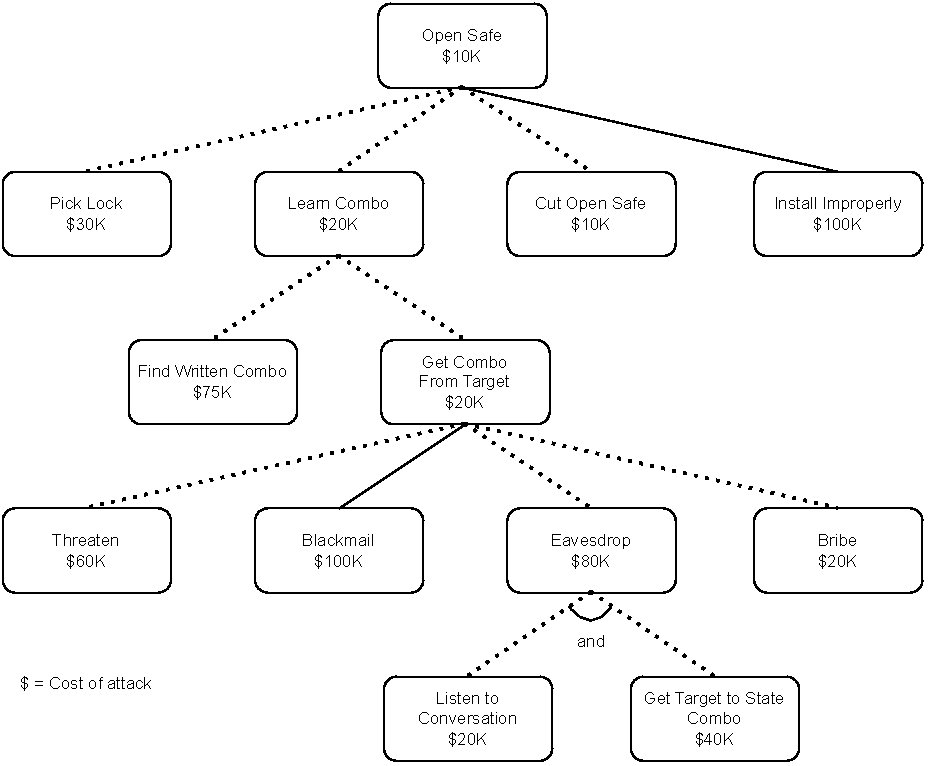
\includegraphics[width=0.8\linewidth]{figures/attack_graph.pdf}
  \caption[Illustration of an attack graph describing a scenario of compromising a safe.] {Illustration of an attack graph describing a scenario of compromising a safe. (adapted from~\cite{schneier1999modeling})~: The root objective \emph{Open Safe} is broken down into four main paths: \emph{Pick Lock} (\$30K), \emph{Learn Combo} (\$20K), \emph{Cut Open Safe} (\$10K), and \emph{Install Improperly} (\$100K) . By default, a node is of type \textsc{OR} (performing one of the children is sufficient);
    when an \emph{and} is indicated, it is an \textsc{AND} (all children are required). The amounts represent estimated costs: for an \textsc{OR}, the cost of the parent is the \emph{minimum} of the child costs;
    for an \textsc{AND}, the costs \emph{are added together}.}
  \label{fig:attack_graphs}
\end{figure}

\

\noindent
\textbf{Attack-defense trees}~: \quad Attack-defense trees~\cite{BKordy2010} (AD trees) are graphical models representing the attacker's objectives and the defender's countermeasures in the form of a tree structure. AD trees provide a more abstract representation of the system and the attackers' objectives, while attack graphs provide a more concrete representation of the system components and their relationships. An example of an AD tree is illustrated in \ autoref{fig:bank_attack_defense_tree}. The root of the \acn{AD} tree represents the ultimate objective of the cyber attackers. The subnodes associated with the branches represent the different attack strategies that the attacker could use to achieve their objective. They may be accompanied by preventive or reactive countermeasures from the defender (firewalls, intrusion detection systems, incident response plans, etc.).
AD trees can be used to identify weaknesses in a system's defense~\cite{BKordy2010}.

\begin{figure}[h!]
  \centering
  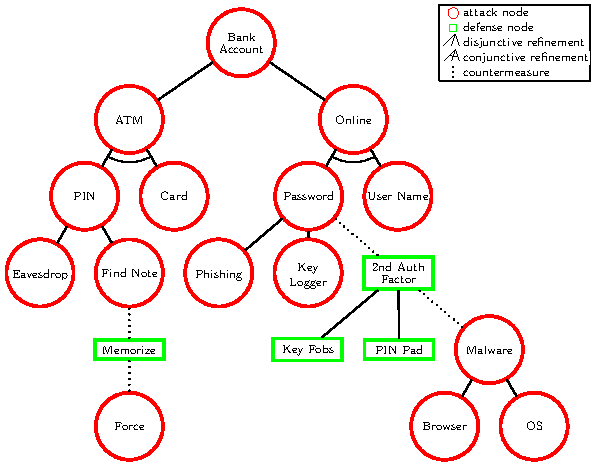
\includegraphics[width=\linewidth]{figures/adt.pdf}
  \caption[Illustration of an ADTree for a bank account attack scenario (taken from~\cite{BKordy2010})]{Illustration of an ADTree describing a bank account attack scenario (taken from~\cite{BKordy2010})~: The account can be accessed via an ATM or online. In the latter case, an ID and password obtained through phishing or a \textit{Key Logger} are required. A countermeasure to these attacks is two-factor authentication using a \textit{fob} key or a PIN code.}
  \label{fig:bank_attack_defense_tree}
\end{figure}

\

\noindent
\textbf{Petri net modeling}: Since Petri nets can be used to describe concurrent processes, some studies have sought to model attackers and defenders in a networked system.
Attacks extracted from databases can be modeled using Petri nets to integrate cyber attackers and cyber defenders, their strategies, and the cost of their actions, as in \cite{MPetty2022}. Petri nets are also useful for modeling structured query language injection attacks to include player strategies. {MPetty2022}. Petri nets are also useful for modeling structured query language injection attacks to include player strategies~\cite {JBland2020}.
They are used as a framework for evaluating and comparing several attack models.
In ~\cite{SYamaguchi2020}, the \textit{Mirai} malware was also expressed as a formal model with Petri nets, allowing the simulation of a battle between a defender agent and \textit{Mirai}.

\

\noindent
\textbf{Game models}~: \quad Some studies have proposed modeling the interactions between attackers and defenders in a network as players in a game, where each player has a set of actions that they can perform.
Notable studies include~: Panfili et al.~\cite{MPanfili2018}, where a multi-agent general-sum game pitting an attacker against a defender is used to find an optimal trade-off between prevention actions and costs; Attiah et al.~\cite {AAttiah2018}, where a dynamic game theoretical framework is proposed to analyze the interactions between the attacker and the defender as a non-cooperative security game; and Xiaolin et al.~\cite{CXiaolin2008}, who use Markov process models to assess risks in networked systems.

\noindent
Some game theory-based approaches fall within the framework of \textquote{partially observable stochastic games} (\acn{POSG}) or, more precisely, \textquote{partially observable decentralized Markov decision processes} (\acn{Dec-POMDP}) . \acn{POSG} and \acn{Dec-POMDP} are both mathematical modeling frameworks for decision-making problems in which agents interact with each other and in a stochastic environment~\cite {beynier2010}. In a \acn{POSG}, a group of agents interacts with a stochastic and partially observable environment. Each agent acts according to its own observations and a local policy. Agents may have different objectives, as each agent has its own reward function and the game is generally assumed to be non-cooperative~\cite{terry2020pettingzoo}. In a \acn{Dec-POMDP}, multiple agents may have a common reward function and may coordinate their actions to achieve a common goal, in particular by being able to communicate~\cite{bernstein2013}.



\subsection{The Dec-PODMP model}\label{sec:dec-podmp}

To apply \acn{MARL} techniques, it is necessary to rely on a Markovian framework to formalize observations, actions, rewards, etc. We rely on the \acn{Dec-POMDP} framework~\cite{Oliehoek2016}. \acn{Dec-POMDP} models allow us to model decentralized coordination between agents in partially observable contexts, making them particularly well suited to the integration of organizational constraints. Unlike \acn{POSG}, \acn{Dec-POMDP} uses a common reward function, thereby promoting collaboration~\cite{Beynier2013}.

A \acn{Dec-POMDP} $d \in D$ (where $D$ is the set of \acparen{Dec-POMDP}) is defined by a 7-tuple $d = (S,\{A_i\},T,R,\{\Omega_i\},O,\gamma)$ where~:
\begin{itemize}
  \item $S = \{s_1, ..., s_{|S|}\}$: the set of possible states.
  \item $A_i = \{a_1^i, ..., a_{|A_i|}^i\}$: the set of possible actions for agent $i$.
  \item $T$ such that $T(s,a,s') = \probP(s'|s,a)$: the conditional transition probability between states.
  \item $R: S \times A \times S \rightarrow \mathbb{R}$: the reward function.
  \item $\Omega_i = \{o_1^i, ..., o_{|\Omega_i|}^i\}$: the set of possible observations for agent $ag_i$.
  \item $O$ such that $O(s',a,o) = \probP(o|s',a)$~: the conditional probability of observing $o$ from $s'$ after performing $a$.
  \item $\gamma \in [0,1]$: the discount factor that describes the importance of future rewards relative to immediate rewards (i.e., the spectrum between greedy behavior and considerate behavior).
\end{itemize}

Considering $m$ \textbf{teams} (or \textbf{groups}), each containing several agents from $\mathcal{A}$, we return to the minimal formalism necessary to solve a \acn{Dec-POMDP} for a given team $i, 0 \leq i \leq m$, composed of $n$ agents~\cite {Beynier2013,Albrecht2024}~:

\begin{itemize}
  \item $\Pi$~: the set of policies. A \textbf{policy} $\pi \in \Pi, \pi~: \Omega \rightarrow A$ is a deterministic function that associates an action with each observation. It represents the internal logic of the agent.
  \item $\Pi_{joint}$~: the set of joint policies. A \textbf{joint policy} $\pi_{joint} \in \Pi_{joint}, \pi_{joint}~: \Omega^n \rightarrow A^n = \Pi^n$ associates an action with each agent based on its observation, and can be seen as the set of policies used by the agents.
  \item $H$: the set of histories. A \textbf{history} on $z \in \mathbb{N}$ steps is a $z$-tuple $h = ((\omega_k, a_k) | k \leq z, \omega \in \Omega, a \in A)$.
  \item $H_{joint}$: the set of joint histories. A \textbf{joint history} over $z$ steps $h_{joint} \in H_{joint}, h_{joint} = \{h_1, h_2, ..., h_n\}$ is the set of histories of the agents.
  \item $U_{joint,i}(\langle \pi_{joint,i}, \pi_{joint,-i} \rangle) : \Pi_{joint} \rightarrow \mathbb{R}$: the \textbf{expected cumulative reward} for team $i$ over a finite horizon, with $\pi_{joint,i}$ the joint policy of team $i$ and $\pi_{joint,-i}$ the joint policies of the other teams (considered fixed).
  \item $BR_{joint,i}(\pi_{joint,i}) = \arg\max_{\pi_{joint,i}} U(\langle \pi_{joint,i}, \pi_{joint,-i} \rangle)$: the \textbf{best responder} $\pi^*_{joint,i}$ such that no policy change would yield a reward greater than $U^*_i = U_{joint,i}(\langle \pi^*_{joint,i}, \pi_{joint,-i} \rangle)$.
  \item $SR_{joint,i}(\pi_{joint,i}, s) = \{\pi_{joint,i} \mid U(\langle \pi_{joint,i}, \pi_{joint,-i} \rangle) \geq s\}$: the \textbf{sufficient response}, i.e., the set of joint policies achieving at least an expected cumulative reward $s \in \mathbb{R}, s \leq U^*_i$.
\end{itemize}

We call the search for a joint policy $\pi^j \in \Pi^j$ such that $U_{joint,i}(\pi^j) \geq s$, achieving an expected cumulative reward at least equal to a threshold $s \in \mathbb{R}$, the \textbf{resolution of the \acn{Dec-POMDP}}.



\subsection{World models}

In \acn{RL}, and in particular in the context of partial observability, \textbf{world models}~\cite{ha2018recurrent, hafner2020dream} or \textit{World Models}\index{World Model} aim to learn internal models that approximate both the dynamics of the transition function and the observation function jointly. \textit{World Models} enable agents to perform planning, improve sampling efficiency, and facilitate safe exploration by allowing the agent to simulate future scenarios. This approach belongs to the \acn{MBRL} ~\cite{moerland2020model} paradigm and is particularly useful for automatically constructing high-fidelity simulation models even in the absence of an explicit representation of the environment.

Formally, at each time step $t$, we denote $\omega_t \in \Omega$ as the current observation, $a_t \in A$ as the action performed, and $\tilde{h}_{t-1} \in \mathcal{H}$ as the recurrent hidden state summarizing the interaction history up to $t-1$. Since observations are generally high-dimensional (e.g., images or complex state vectors), an encoder $Enc: \Omega \rightarrow Z$ is applied to project the observations into a compact latent space $Z$, with $z_t = Enc(\omega_t)$, where $\dim(Z) \ll \dim(\Omega)$.

The main temporal structure is modeled using a \textbf{Recurrent Latent Dynamic Model (\acparen{RLDM})}~\cite{hafner2020dream} $\mathcal{T}^{z} = f(g(h_{t-1}, z_t, a_t))$, which predicts the next latent state $\hat{z}_{t+1}$ by updating the recurrent state via $f$ and applying latent dynamics via $g$~:
\[
  \hspace{4cm}h_t = f(h_{t-1}, z_t, a_t), \quad \hat{z}_{t+1} = g(h_t)
\]
where $f(\cdot)$ typically corresponds to a recurrent neural network \acn{RNN}\index{RNN} (e.g., an \acparen{LSTM}~\cite{hochreiter1997long}\index{LSTM}) applied to the concatenation of $h_{t-1} $, $z_t$ and $a_t$, and $g(\cdot)$ is a function (often implemented by an \acparen{MLP}\index{MLP}) mapping the recurrent state to the latent representation of the next observation.

The predicted latent state is then decoded by $Dec: Z \rightarrow \Omega$ to produce the predicted observation $\hat{\omega}_{t+1} = Dec(\hat{z}_{t+1})$. The entire model is trained jointly to minimize both the \emph{reconstruction loss} $\|\omega_{t+1} - \hat{\omega}_{t+1}\|$ in the observation space, and optionally a latent prediction loss to stabilize the learning of the latent dynamics.

The recurrent hidden state $\tilde{h}_t$ acts as a compact summary of the complete interaction history up to time $t$, thus avoiding the need to explicitly store long observation-action sequences.

For the sake of brevity, we define the complete composition that directly associates the current observation, action, and recurrent state with the next predicted observation in the form of the Observation Prediction Model (\acparen{OPM})\index{Observation Prediction Model (OPM)}~:
\[
  \hspace{2cm}\mathcal{T}(h_{t-1}, \omega_t, a_t)~:= Dec(g(f(h_{t-1}, Enc(\omega_t), a_t))) = \hat{\omega}_{t+1}.
\]

\begin{figure}[h!]
  \centering
  \resizebox{\textwidth}{!}{%
    


\tikzset{every picture/.style={line width=0.75pt}} %set default line width to 0.75pt        

\begin{tikzpicture}[x=0.75pt,y=0.75pt,yscale=-1,xscale=1]
    %uncomment if require: \path (0,2102); %set diagram left start at 0, and has height of 2102

    %Straight Lines [id:da7945271061326031] 
    \draw    (100,1800) -- (111.5,1800) ;
    \draw [shift={(113.5,1800)}, rotate = 180] [color={rgb, 255:red, 0; green, 0; blue, 0 }  ][line width=0.75]    (6.56,-1.97) .. controls (4.17,-0.84) and (1.99,-0.18) .. (0,0) .. controls (1.99,0.18) and (4.17,0.84) .. (6.56,1.97)   ;
    %Straight Lines [id:da710289636295716] 
    \draw    (100,1835) -- (188,1834) -- (188,1820) ;
    \draw [shift={(188,1818)}, rotate = 90] [color={rgb, 255:red, 0; green, 0; blue, 0 }  ][line width=0.75]    (6.56,-1.97) .. controls (4.17,-0.84) and (1.99,-0.18) .. (0,0) .. controls (1.99,0.18) and (4.17,0.84) .. (6.56,1.97)   ;
    %Straight Lines [id:da9775676154282154] 
    \draw    (146.38,1800) -- (160,1800) ;
    \draw [shift={(162,1800)}, rotate = 180] [color={rgb, 255:red, 0; green, 0; blue, 0 }  ][line width=0.75]    (7.65,-2.3) .. controls (4.86,-0.97) and (2.31,-0.21) .. (0,0) .. controls (2.31,0.21) and (4.86,0.98) .. (7.65,2.3)   ;
    %Straight Lines [id:da789934339782699] 
    \draw    (100,1766) -- (122,1766) ;
    \draw [shift={(124,1766)}, rotate = 180] [color={rgb, 255:red, 0; green, 0; blue, 0 }  ][line width=0.75]    (6.56,-1.97) .. controls (4.17,-0.84) and (1.99,-0.18) .. (0,0) .. controls (1.99,0.18) and (4.17,0.84) .. (6.56,1.97)   ;
    %Shape: Trapezoid [id:dp2317709974845179] 
    \draw   (123.84,1754.74) -- (142.07,1760.21) -- (142.07,1771.42) -- (123.84,1776.88) -- cycle ;
    %Straight Lines [id:da7383754609221514] 
    \draw    (142,1766) -- (188,1766) -- (188,1780) ;
    \draw [shift={(188,1782)}, rotate = 270] [color={rgb, 255:red, 0; green, 0; blue, 0 }  ][line width=0.75]    (6.56,-1.97) .. controls (4.17,-0.84) and (1.99,-0.18) .. (0,0) .. controls (1.99,0.18) and (4.17,0.84) .. (6.56,1.97)   ;
    %Straight Lines [id:da49394763541143527] 
    \draw    (216,1800) -- (237.33,1799.94) ;
    \draw [shift={(239.33,1799.94)}, rotate = 179.85] [color={rgb, 255:red, 0; green, 0; blue, 0 }  ][line width=0.75]    (6.56,-1.97) .. controls (4.17,-0.84) and (1.99,-0.18) .. (0,0) .. controls (1.99,0.18) and (4.17,0.84) .. (6.56,1.97)   ;
    %Straight Lines [id:da8738633046359771] 
    \draw    (265.89,1800.03) -- (284.72,1800.03) ;
    \draw [shift={(286.72,1800.03)}, rotate = 180] [color={rgb, 255:red, 0; green, 0; blue, 0 }  ][line width=0.75]    (6.56,-1.97) .. controls (4.17,-0.84) and (1.99,-0.18) .. (0,0) .. controls (1.99,0.18) and (4.17,0.84) .. (6.56,1.97)   ;
    %Straight Lines [id:da3021616845453272] 
    \draw    (302,1800) -- (320.83,1800) ;
    \draw [shift={(322.83,1800)}, rotate = 180] [color={rgb, 255:red, 0; green, 0; blue, 0 }  ][line width=0.75]    (6.56,-1.97) .. controls (4.17,-0.84) and (1.99,-0.18) .. (0,0) .. controls (1.99,0.18) and (4.17,0.84) .. (6.56,1.97)   ;
    %Straight Lines [id:da8984410115217915] 
    \draw    (346,1800) -- (353.4,1800) -- (365.04,1800) ;
    \draw [shift={(367.04,1800)}, rotate = 180] [color={rgb, 255:red, 0; green, 0; blue, 0 }  ][line width=0.75]    (6.56,-1.97) .. controls (4.17,-0.84) and (1.99,-0.18) .. (0,0) .. controls (1.99,0.18) and (4.17,0.84) .. (6.56,1.97)   ;
    %Shape: Trapezoid [id:dp37639710819638017] 
    \draw   (423.61,1812) -- (405.38,1806.53) -- (405.38,1795.32) -- (423.61,1789.86) -- cycle ;
    %Straight Lines [id:da10289425963982124] 
    \draw    (384,1800) -- (403.04,1800) ;
    \draw [shift={(405.04,1800)}, rotate = 180] [color={rgb, 255:red, 0; green, 0; blue, 0 }  ][line width=0.75]    (6.56,-1.97) .. controls (4.17,-0.84) and (1.99,-0.18) .. (0,0) .. controls (1.99,0.18) and (4.17,0.84) .. (6.56,1.97)   ;
    %Straight Lines [id:da12692360321469986] 
    \draw    (424,1800) -- (443.04,1800) ;
    \draw [shift={(445.04,1800)}, rotate = 180] [color={rgb, 255:red, 0; green, 0; blue, 0 }  ][line width=0.75]    (6.56,-1.97) .. controls (4.17,-0.84) and (1.99,-0.18) .. (0,0) .. controls (1.99,0.18) and (4.17,0.84) .. (6.56,1.97)   ;
    %Shape: Trapezoid [id:dp27180057752038367] 
    \draw   (217.23,1670.74) -- (235.46,1676.21) -- (235.46,1687.42) -- (217.23,1692.88) -- cycle ;
    %Shape: Trapezoid [id:dp9437628483591106] 
    \draw   (309.61,1695) -- (291.38,1689.53) -- (291.38,1678.32) -- (309.61,1672.86) -- cycle ;
    %Straight Lines [id:da19635385567867214] 
    \draw    (310,1683) -- (328,1683) ;
    \draw [shift={(330,1683)}, rotate = 180] [color={rgb, 255:red, 0; green, 0; blue, 0 }  ][line width=0.75]    (6.56,-1.97) .. controls (4.17,-0.84) and (1.99,-0.18) .. (0,0) .. controls (1.99,0.18) and (4.17,0.84) .. (6.56,1.97)   ;
    %Straight Lines [id:da6136759960935583] 
    \draw    (196,1683) -- (214.83,1683) ;
    \draw [shift={(216.83,1683)}, rotate = 180] [color={rgb, 255:red, 0; green, 0; blue, 0 }  ][line width=0.75]    (6.56,-1.97) .. controls (4.17,-0.84) and (1.99,-0.18) .. (0,0) .. controls (1.99,0.18) and (4.17,0.84) .. (6.56,1.97)   ;
    %Straight Lines [id:da5198115307428596] 
    \draw    (236,1683) -- (255.04,1683) ;
    \draw [shift={(257.04,1683)}, rotate = 180] [color={rgb, 255:red, 0; green, 0; blue, 0 }  ][line width=0.75]    (6.56,-1.97) .. controls (4.17,-0.84) and (1.99,-0.18) .. (0,0) .. controls (1.99,0.18) and (4.17,0.84) .. (6.56,1.97)   ;
    %Straight Lines [id:da6362560665768464] 
    \draw    (270,1683) -- (289.04,1683) ;
    \draw [shift={(291.04,1683)}, rotate = 180] [color={rgb, 255:red, 0; green, 0; blue, 0 }  ][line width=0.75]    (6.56,-1.97) .. controls (4.17,-0.84) and (1.99,-0.18) .. (0,0) .. controls (1.99,0.18) and (4.17,0.84) .. (6.56,1.97)   ;
    %Shape: Rectangle [id:dp3864765488610862] 
    \draw  [color={rgb, 255:red, 74; green, 144; blue, 226 }  ,draw opacity=1 ][dash pattern={on 0.84pt off 2.51pt}] (70,1720) -- (475,1720) -- (475,1855) -- (70,1855) -- cycle ;
    %Shape: Rectangle [id:dp17767261593347572] 
    \draw  [color={rgb, 255:red, 65; green, 117; blue, 5 }  ,draw opacity=1 ][dash pattern={on 0.84pt off 2.51pt}] (175,1660) -- (355,1660) -- (355,1700) -- (175,1700) -- cycle ;
    %Shape: Polygon [id:ds8294746409292746] 
    \draw  [color={rgb, 255:red, 208; green, 2; blue, 27 }  ,draw opacity=1 ][dash pattern={on 0.84pt off 2.51pt}] (390,1845) -- (75,1845) -- (75,1780.92) -- (150,1780) -- (150,1750) -- (390,1750) -- cycle ;


    % Text Node
    \draw (333.5,1764.5) node  [color={rgb, 255:red, 208; green, 2; blue, 27 }  ,opacity=1 ] [align=left] {\footnotesize \textbf{\textit{RDLM}}};
    % Text Node
    \draw (317.5,1734.5) node  [color={rgb, 255:red, 74; green, 144; blue, 226 }  ,opacity=1 ] [align=left] {\footnotesize Modèle de prédiction d'observation (\textbf{\textit{OPM}})};
    % Text Node
    \draw (264.5,1645.5) node  [color={rgb, 255:red, 65; green, 117; blue, 5 }  ,opacity=1 ] [align=left] {{\footnotesize \textbf{Auto-encodeur}}};
    % Text Node
    \draw (189.5,1683) node  [font=\tiny] [align=left] {$\displaystyle \omega _{t}$};
    % Text Node
    \draw (340,1682) node  [font=\tiny] [align=left] {$\displaystyle \hat{\omega }_{t}$};
    % Text Node
    \draw (301.5,1679.5) node   [align=left] {{\tiny Dec}};
    % Text Node
    \draw (225.38,1676.5) node   [align=left] {{\tiny Enc}};
    % Text Node
    \draw (264.5,1684) node  [font=\tiny] [align=left] {$\displaystyle z_{t}$};
    % Text Node
    \draw (456.54,1799) node  [font=\tiny] [align=left] {$\displaystyle \hat{\omega }_{t+1}$};
    % Text Node
    \draw (415.5,1796.5) node   [align=left] {{\tiny Dec}};
    % Text Node
    \draw (375.5,1799) node  [font=\tiny] [align=left] {$\displaystyle z_{t+1}$};
    % Text Node
    \draw (132,1760.5) node   [align=left] {{\tiny Enc}};
    % Text Node
    \draw (295,1798) node  [font=\tiny] [align=left] {$\displaystyle \tilde{h}_{t}$};
    % Text Node
    \draw    (239.48,1779) -- (265.48,1779) -- (265.48,1817) -- (239.48,1817) -- cycle  ;
    \draw (252.48,1798) node  [font=\tiny] [align=left] {\begin{minipage}[lt]{14.99pt}\setlength\topsep{0pt}
            \begin{center}
                \phantom{X}\\\textit{RNN}
            \end{center}

        \end{minipage}};
    % Text Node
    \draw  [color={rgb, 255:red, 255; green, 255; blue, 255 }  ,draw opacity=1 ][fill={rgb, 255:red, 255; green, 255; blue, 255 }  ,fill opacity=1 ]  (157.5,1757) -- (174.5,1757) -- (174.5,1773) -- (157.5,1773) -- cycle  ;
    \draw (166,1765) node  [font=\tiny] [align=left] {$\displaystyle z_{t}$};
    % Text Node
    \draw    (162,1782) -- (216,1782) -- (216,1818) -- (162,1818) -- cycle  ;
    \draw (189,1800) node  [font=\tiny] [align=left] {\begin{minipage}[lt]{34pt}\setlength\topsep{0pt}
            \begin{center}
                \phantom{X}\\\textit{concatenate}
            \end{center}

        \end{minipage}};
    % Text Node
    \draw (91,1833) node  [font=\tiny] [align=left] {$\displaystyle \tilde{h}_{t-1}$};
    % Text Node
    \draw (91.5,1801) node  [font=\tiny] [align=left] {$\displaystyle a_{t}$};
    % Text Node
    \draw (91.5,1766) node  [font=\tiny] [align=left] {$\displaystyle \omega _{t}$};
    % Text Node
    \draw    (322.5,1792) -- (345.5,1792) -- (345.5,1807) -- (322.5,1807) -- cycle  ;
    \draw (334,1799.5) node  [font=\tiny] [align=left] {MLP};
    % Text Node
    \draw    (113,1788) -- (146,1788) -- (146,1813) -- (113,1813) -- cycle  ;
    \draw (129.5,1800.5) node  [font=\tiny] [align=left] {one-hot\\encode};


\end{tikzpicture}
  }
  \caption{Illustration of the architecture of a \textit{World Model} comprising the Autoencoder and the OPM}
  \label{fig:single_agent_world_model}
\end{figure}

\autoref{fig:single_agent_world_model} illustrates the architecture of a \textit{World Model} comprising the Autoencoder and the \acn{OPM}.

\textbf{Autoencoder training phase:} An autoencoder, such as a \acn{VAE}, is first trained to encode and decode observations into latent representations. The goal is to minimize the gap between the actual observations and the decoded observations.

\textbf{Initialization and transition processing:} Initially, the recurrent hidden state $\tilde{h}_{t-1}$ is initialized to the zero vector. For each history and each transition, an input vector is constructed by concatenating three elements: the representation of the observation $z_t$, the action $a_t$ (after one-hot encoding), and the recurrent hidden state $\tilde{h}_{t-1}$.

\textbf{How \acn{RLDM} works:} This input vector is processed by \acn{RLDM} in a two-step process. First, it passes through the \acn{RNN}, which updates the recurrent hidden state with the new transitions to obtain $\hat{h}_t$. Then, this vector is passed to an \acn{MLP}, which determines the latent representation of the next observation $\hat{z}_{t+1}$.

\textbf{Training and prediction:} The \acn{RLDM} is trained to minimize the quadratic error between the predicted observation and the actual observation. Once training is complete, a latent representation of a predicted observation can be decoded into a predicted observation $\omega_{t+1}$.

\section{Constrained reinforcement learning (CRL)}

Constrained reinforcement learning aims to equip agents with the ability to optimize their behavior while respecting additional requirements, such as safety, fairness, or organizational rules. This section presents the main theoretical and technical frameworks for explicitly or implicitly integrating constraints into the learning process, drawing on extensions of classical \acn{RL}, Safe \acn{RL} methods, and organizational guidance mechanisms.

\subsection {Multi-agent reinforcement learning}
% Recall the basics of \acn{MARL} and explain using the \acn{Dec-POMDP} formalism defined above

Reinforcement learning (\acparen{RL})\index{Reinforcement learning (RL)} is a formal framework in which an agent learns to act in an unknown environment by interacting with it. At each step, the agent observes a state (or partial observation), executes an action, receives a reward, and perceives a new state. The goal is to maximize the long-term cumulative reward, typically modeled by an expected return function.

Formally, the problem is often represented as a Markov decision process (\acparen{MDP}), defined by a quintuple $\langle S, A, T, R, \gamma \rangle$, where~:
\begin{itemize}
  \item $S$ is the set of states~;
  \item $A$ is the set of possible actions;
  \item $T: S \times A \rightarrow \mathcal{P}(S)$ is the transition function;
  \item $R: S \times A \rightarrow \mathbb{R}$ is the reward function;
  \item $\gamma \in [0,1]$ is the discount factor.
        \end {itemize}

        The agent learns a policy $\pi~: S \rightarrow A$ (or stochastic) that maximizes the sum of expected rewards. In the partially observable case (\acparen{POMDP}), states are inaccessible, and the agent acts based on observations and history.


        In the multi-agent case, several agents interact simultaneously with the environment. The problem becomes more complex because:
        \begin{itemize}
          \item \textbf{The environment becomes non-stationary}: each agent modifies the environment and disrupts the learning of others;
          \item \textbf{Exploration becomes joint}: the consequences of an action may depend on the behavior of others;
          \item \textbf{Attribution credit is difficult}: linking a reward to the action of a specific agent becomes ambiguous.
        \end{itemize}

        \acn{MARL}\index{Multi-Agent Reinforcement Learning (MARL)} addresses these difficulties by adapting \acn{RL} methods to this context. Two main approaches can be distinguished:
        \begin {itemize}
  \item \textbf{Independent Learners}~: each agent learns its policy by considering others as part of the environment (simplifies implementation, but generates instability);
  \item \textbf{Centralized Training with Decentralized Execution (\acparen{CTDE})}~: learning is done in a coordinated manner, with access to global information (states, rewards), but the final policies must be able to execute autonomously.
        \end {itemize}


        MARL has been successfully applied in several areas: robot coordination, cooperative games, traffic management, energy systems, etc. In the context of cyberdefense, it offers interesting potential for designing adaptive policies capable of responding to dynamic and partially observed threats.

        However, several limitations remain:
        \begin{itemize}
          \item \textbf{The difficulty of convergence} in complex or competitive environments;
          \item \textbf{The lack of guarantees of safety or compliance with constraints};
          \item \textbf{The low explainability of learned policies}, often represented by neural networks;
          \item \textbf{The absence of explicit organizational structuring} in existing architectures.
        \end{itemize}

        These limitations motivate closer integration between learning methods and organizational models, which we will explore in the following sections.



        \subsection{Constrained MDPs, Safe RL, and Implicit Guidance}

        \noindent
        One of the main challenges of \acn{RL} applied to critical environments
        such as cyber defense lies in the ability to guarantee the safety of learned policies,
        while maintaining the adaptability inherent in connectionist learning.
        Indeed, classical policy optimization methods aim to maximize a cumulative reward,
        without taking into account additional constraints (security, organizational rules, fairness, etc.).
        To overcome this limitation, numerous extensions have been proposed, grouped under the banner
        of \textit{Safe RL} and \textit{Constrained MDPs}.

        \paragraph{Constrained Markov Decision Processes (CMDP).}
        A \textit{CMDP}~\cite{altman1999constrained} extends the classical \acn{MDP} framework by incorporating
        a set of costs $C_i$ subject to maximum bounds $d_i$.
        A \acn{CMDP} is defined by a quintuple
        $\langle S, A, T, R, \{C_i\}, \gamma \rangle$,
        where $(S,A,T,R,\gamma)$ corresponds to the standard \acn{MDP}, and where
        each $C_i : S \times A \rightarrow \mathbb {R}$ represents a constrained cost function.
        The objective then becomes~:
        \[
          \hspace{1cm}\max_{\pi} \;\; \mathbb{E}\!\left[\sum_{t=0}^\infty \gamma^t R(s_t,a_t)\right]
          \quad \text {s.c.} \quad
          \mathbb{E}\!\left[\sum_{t=0}^\infty \gamma^t C_i(s_t,a_t)\right] \leq d_i, \;\; \forall i
        \]
        This formalism naturally generalizes planning problems where certain properties
        (safety, consumption, risk) must be respected in addition to reward maximization.

        \paragraph{Safe RL and constrained optimizations.}
        In line with \acn{CMDP}, several methods have been developed to solve constrained problems in a practical way.
        Among the most notable are:
        \begin{itemize}
          \item \textbf{Constrained Policy Optimization (\acn{CPO})}~\cite{achiam2017constrained},
                which extends \acn{TRPO} by ensuring,
                via Lagrangian optimization, that constraints are
                not violated beyond a fixed threshold.
                This method provides partial safety guarantees during training.
          \item \textbf{Deep Constrained Q-Learning (\acn{DCQL})}~\cite{kalweit2020deep},
                which adapts deep Q-Learning to constrained environments
                by integrating Lagrange multipliers into the approximation
                of the value function.
        \end{itemize}

        \paragraph{Implicit guidance.}
        Beyond \acn{CMDP}, other works propose to indirectly influence
        the behavior of agents through flexible guidance mechanisms,
        without explicit constraints~:
        \begin{itemize}
          \item \textbf{Reward shaping}~\cite{ng1999policy}~: modification of the
                reward function to encourage certain behaviors (e.g., cooperation,
                compliance with protocols).
          \item \textbf{Shielding}~\cite{amodei2016concrete}~: a priori or a posteriori filtering
                of dangerous actions using a safety model,
                preventing the agent from executing prohibited behaviors.
          \item \textbf{Human feedback}~\cite{warnell2018deep}~: incorporation of corrections
                or preferences provided by a human operator,
                allowing interactive guidance of learning.
        \end{itemize}

        CMDPs and Safe RL provide a first level of theoretical guarantees regarding compliance with constraints, but these generally remain limited to local constraints (at the action or trajectory level) and are numerical in nature. Implicit guidance mechanisms offer considerable flexibility, but do not provide formal guarantees. Furthermore, these approaches are not yet adapted to the multi-agent context, which would require an extension of the formalism to integrate interactions between agents. Nevertheless, they constitute an important basis for considering the integration of more expressive organizational constraints, which we will seek to articulate later with symbolic models such as $\mathcal{M}OISE^+$.

        \subsection{The $\mathcal{M}OISE^+$ model}
        % Organizational models (e.g., MOISE+)
        % Roles, Missions, Permissions, Obligations (R-M-P-O)

        \begin{figure}[h!]
          \centering
          


\tikzset{every picture/.style={line width=0.75pt}} %set default line width to 0.75pt        

\begin{tikzpicture}[x=0.75pt,y=0.75pt,yscale=-1,xscale=1]
%uncomment if require: \path (0,1656); %set diagram left start at 0, and has height of 1656

%Shape: Rectangle [id:dp6756844921493015] 
\draw  [fill={rgb, 255:red, 248; green, 231; blue, 28 }  ,fill opacity=1 ] (46,1204) -- (214,1204) -- (214,1424) -- (46,1424) -- cycle ;
%Shape: Rectangle [id:dp3759944257810566] 
\draw  [fill={rgb, 255:red, 80; green, 227; blue, 194 }  ,fill opacity=1 ] (390,1204) -- (556,1204) -- (556,1424) -- (390,1424) -- cycle ;
%Shape: Rectangle [id:dp28244406216006945] 
\draw  [fill={rgb, 255:red, 144; green, 19; blue, 254 }  ,fill opacity=1 ] (218,1234) -- (386,1234) -- (386,1338) -- (218,1338) -- cycle ;
%Shape: Rectangle [id:dp32232123359581766] 
\draw   (42,1176) -- (562,1176) -- (562,1428) -- (42,1428) -- cycle ;
%Shape: Rectangle [id:dp7605706269262755] 
\draw  [fill={rgb, 255:red, 74; green, 144; blue, 226 }  ,fill opacity=1 ] (396,1286) -- (550,1286) -- (550,1418) -- (396,1418) -- cycle ;
%Shape: Rectangle [id:dp33110985390647496] 
\draw   (52,1294) -- (210,1294) -- (210,1418) -- (52,1418) -- cycle ;
%Shape: Rectangle [id:dp8653560038381976] 
\draw  [fill={rgb, 255:red, 245; green, 166; blue, 35 }  ,fill opacity=1 ] (52,1294) -- (210,1294) -- (210,1418) -- (52,1418) -- cycle ;
%Straight Lines [id:da09781093164567278] 
\draw    (412,1350) -- (353.61,1307.18) ;
\draw [shift={(352,1306)}, rotate = 36.25] [color={rgb, 255:red, 0; green, 0; blue, 0 }  ][line width=0.75]    (10.93,-3.29) .. controls (6.95,-1.4) and (3.31,-0.3) .. (0,0) .. controls (3.31,0.3) and (6.95,1.4) .. (10.93,3.29)   ;
%Straight Lines [id:da3938396723807833] 
\draw    (122,1334) -- (264.04,1304.41) ;
\draw [shift={(266,1304)}, rotate = 168.23] [color={rgb, 255:red, 0; green, 0; blue, 0 }  ][line width=0.75]    (10.93,-3.29) .. controls (6.95,-1.4) and (3.31,-0.3) .. (0,0) .. controls (3.31,0.3) and (6.95,1.4) .. (10.93,3.29)   ;
%Shape: Rectangle [id:dp269311335478327] 
\draw  [color={rgb, 255:red, 208; green, 2; blue, 27 }  ,draw opacity=1 ][line width=1.5]  (66,1322) -- (122,1322) -- (122,1334) -- (66,1334) -- cycle ;
%Shape: Rectangle [id:dp7449860119164387] 
\draw  [color={rgb, 255:red, 208; green, 2; blue, 27 }  ,draw opacity=1 ][line width=1.5]  (412,1342) -- (488,1342) -- (488,1354) -- (412,1354) -- cycle ;


% Text Node
\draw (472.5,1237.41) node   [align=left] {\begin{minipage}[lt]{112.2pt}\setlength\topsep{0pt}
\begin{center}
\textbf{{\small Functional Specs.}}
\end{center}
{\small  - Social schemes $\displaystyle \mathcal{SCH}$}\\{\small  - Social preferences $\displaystyle \mathcal{SP}$}
\end{minipage}};
% Text Node
\draw (474,1355) node   [align=left] {\begin{minipage}[lt]{103.36pt}\setlength\topsep{0pt}
\begin{center}
\textbf{{\small Social Scheme.}}\\{\small \textbf{Specs. }$\displaystyle (\mathcal{SCH})$}
\end{center}
{\small  - Goals $\displaystyle \mathcal{G}$}\\{\small  - Missions $\displaystyle \mathcal{M}$}\\{\small  - Plans $\displaystyle \mathcal{P}$}\\{\small  - Mission to goals \ $\displaystyle mo$}\\\\{\small  ...}
\end{minipage}};
% Text Node
\draw (131,1356) node   [align=left] {\begin{minipage}[lt]{104.72pt}\setlength\topsep{0pt}
\begin{center}
{\small \textbf{Group Specs. }$\displaystyle (\mathcal{G} r)$}
\end{center}
{\small  - Roles $\displaystyle \mathcal{R}$}\\{\small  - Sub-groups $\displaystyle \mathcal{SG} \ \subset \mathcal{G} r$}\\{\small  - Links $\displaystyle \mathcal{L}$}\\{\small  - Compatibilities $\displaystyle \mathcal{C}$}\\\\{\small  ...}
\end{minipage}};
% Text Node
\draw (181,1177) node [anchor=north west][inner sep=0.75pt]   [align=left] {\begin{minipage}[lt]{162.41pt}\setlength\topsep{0pt}
\begin{center}
{\small \textbf{Organisational Specs. }$\displaystyle \mathcal{M}\boldsymbol{OISE^{+}}$($\displaystyle \mathbf{OS}$)}
\end{center}

\end{minipage}};
% Text Node
\draw (300,1269.09) node   [align=left] {\begin{minipage}[lt]{92.48pt}\setlength\topsep{0pt}
\begin{center}
\textbf{{\small Deontic Specs.}}
\end{center}
{\small  - Permissions $\displaystyle \mathcal{PER}$}\\{\small  - Obligations $\displaystyle \mathcal{OBL}$}
\end{minipage}};
% Text Node
\draw (130.5,1245.69) node   [align=left] {\begin{minipage}[lt]{112.2pt}\setlength\topsep{0pt}
\begin{center}
\textbf{{\small Structural Specs.}}
\end{center}
{\small  - Root-groups $\displaystyle \mathcal{G} r$}\\{\small  - Roles $\displaystyle \mathcal{R}_{ss}$}\\{\small  - Roles inheritance $\displaystyle \mathcal{IR}$}
\end{minipage}};


\end{tikzpicture}
          \caption{Overview of the $\mathcal{M}OISE^+$ model}
          \label{fig:moise_model}
        \end{figure}

        The $\mathcal{M}OISE^+$~\citep{Hubner2002}\index{MOISE+} model provides an advanced formal description of an organization, particularly for the formal description of agent policies (via plans). It explicitly takes into account social aspects between agents, whereas \acn{AGR} focuses on the integration of design-oriented norms. In addition, it offers a sufficiently detailed view of the organization to be understood from different perspectives. A visual representation of the formal elements of this model is given in \autoref{fig:moise_model}
        Based on the formalism of $\mathcal{M}OISE^+$~\citep{hubner2007moise}, we do not detail the main minimal elements here.

        \

        \noindent \textbf {Organizational specifications}~: Organizational specifications include all structural, functional, and deontic specifications \quad $\mathcal{OS} = \langle \mathcal{SS}, \mathcal{FS}, \mathcal{DS} \rangle$, the set of organizational specifications, where $\mathcal{SS}$ are the \textbf{structural specifications}, $\mathcal{FS}$ the \textbf {functional specifications}, and $\mathcal{DS}$ are the \textbf{deontic specifications}.

        \

        \noindent \textbf{Structural Specifications}~: These define the structure of the organization by describing the roles, groups, and social links that are permitted, specifying how agents can interact. They are denoted \quad $\mathcal{SS} = \langle \mathcal{R}, \mathcal{IR}, \mathcal{G} \rangle$, where~:

        \begin{itemize}
          \item $\mathcal{R}_{ss}$: the set of roles (denoted $\rho \in \mathcal{R}$);
          \item $\mathcal{IR}: \mathcal{R} \rightarrow \mathcal{R}$: the inheritance relationship between roles ($\mathcal {IR}(\rho_1) = \rho_2$ means that $\rho_1$ inherits from $\rho_2$, also denoted $\rho_1 \sqsubset \rho_2$)~;
          \item $RG \subseteq GR$~: the set of root groups, $GR = \langle \mathcal{R}, \mathcal{SG}, \mathcal{L}^{intra}, \mathcal{L}^{inter}, \mathcal{C}^{intra}, \mathcal{C}^{inter}, np, ng \rangle$, the set of groups, where:
                \begin{itemize}
                  \item $\mathcal{R} \subseteq \mathcal{R}_{ss}$: the set of non-abstract roles;
                  \item $\mathcal{SG} \subseteq \mathcal{GR}$: the set of subgroups;
                  \item $\mathcal{L} = \mathcal{R} \times \mathcal{R} \times \mathcal{TL}$: the set of links. A link is a triplet $(\rho_s,\rho_d,t) \in \mathcal{L}$ (also denoted $link(\rho_s,\rho_d,t)$), where $\rho_s$ is the source role, $\rho_d$ is the destination role, and $t \in \mathcal{TL}, \mathcal{TL} = \{acq, com, aut\}$ is the link type:
                        \begin{itemize}
                          \item $t = acq$ (acquaintance): agents playing $\rho_s$ can identify agents playing $\rho_d$;
                          \item $t = com$ (communication): agents playing $\rho_s$ can communicate with those playing $\rho_d$;
                          \item $t = aut$ (authority): agents playing $\rho_s$ can exercise authority over those playing $\rho_d$.
                                This link requires acquaintance and communication links.
                        \end{itemize}
                  \item $\mathcal{L}^{intra} \subseteq \mathcal{L}$: set of intra-group links;
                  \item $\mathcal{L}^{inter} \subseteq \mathcal{L} $~: set of inter-group links~;
                  \item $\mathcal{C} = \mathcal{R} \times \mathcal {R}$: the set of compatibilities. A compatibility is a pair $(\rho_a, \rho_b) \in \mathcal{C}$ (also denoted $\rho_a \bowtie \rho_b$), meaning that an agent playing $\rho_a$ can also play $\rho_b$;
                  \item $\mathcal{C}^{intra} \subseteq \mathcal{C}$: set of intra-group compatibilities;
                  \item $\mathcal{C}^{inter} \subseteq \mathcal{C}$: set of inter-group compatibilities;
                  \item $np: \mathcal{R} \rightarrow \mathbb{N} \times \mathbb{N}$: relation giving the cardinality of the number of agents per role;
                  \item $ng: \mathcal{SG} \rightarrow \mathbb{N} \times \mathbb{N}$: relation giving the cardinality of each subgroup.
                \end{itemize}
        \end{itemize}

        \medskip

        \noindent \textbf{Functional Specifications}: These describe the collective objectives and their breakdown into sub-objectives, indicating which ones must be accomplished and in what order. They are denoted
        \quad $\mathcal{FS} = \langle \mathcal{SCH}, \mathcal{PO} \rangle$, where:

        \begin {itemize}
  \item $\mathcal{SCH} = \langle\mathcal{G}, \mathcal{M}, \mathcal{P}, mo, nm \rangle$: the set of \textbf{social schemes}, where:
        \begin{itemize}
          \item $\mathcal{G}$: the set of global objectives;
          \item $\mathcal{M}$: the set of missions;
          \item $\mathcal{P} = \langle \mathcal{G}, \{\mathcal{G}\}^s, OP, [0,1] \rangle, s \in \mathbb{N}^*$: set of plans that define the tree of objectives.
                A plan $p \in \mathcal{P}$ is a 4-tuple $p = (g_f, \{g_i\}_{0 \leq i \leq s}, op, p)$, where $g_f \in \mathcal{G}$ is an objective, the $g_i \in \mathcal{G}$ are sub-objectives, $op \in OP = \{sequence, choice, parallel\}$ is an operator, and $p \in [0,1]$ is a probability of success~:
                \begin{itemize}
                  \item $op = sequence$: the $g_i$ must be achieved in a specific order;
                  \item $op = choice$: only one $g_i$ must be achieved;
                  \item $op = parallel$: the $g_i$ can be achieved in parallel or sequentially.
                \end{itemize}
          \item $mo: \mathcal{M} \rightarrow \mathbb{P}(\mathcal{G})$: relation linking a mission to a set of objectives;
          \item $nm: \mathcal{M} \rightarrow \mathbb{N} \times \mathbb{N}$: cardinality of the number of agents assigned to a mission.
                \end {itemize}
          \item $\mathcal{PO}: \mathcal{M} \times \mathcal{M} $~: set of \textbf{preference orders}. A preference order is a pair $(m_1, m_2)$ (also denoted $m_1 \prec m_2$) meaning that if an agent can commit to both $m_1$ and $m_2$, they will have a social preference for $m_1$.
        \end{itemize}

        \medskip

        \noindent \textbf{Deontic specifications}~: These state the normative rules linking roles to missions.
        They regulate who must, can, or cannot perform certain missions. They are denoted \quad $\mathcal{DS} = \langle \mathcal{OBL}, \mathcal{PER} \rangle$, the set of deontic specifications, where~:
        %
        \begin{itemize}
          \item $\mathcal{TC}$: set of \textbf{temporal constraints}.
                A constraint $tc \in \mathcal{TC}$ indicates the periods during which a permission or obligation is valid ($Any \in \mathcal{TC}$ means all the time);
          \item $\mathcal{OBL}: \mathcal{R} \times \mathcal{M} \times \mathcal{TC}$: set of \textbf{obligations}. An obligation is a triplet $(\rho_a, m, tc)$ (also denoted $obl(\rho_a, m, tc)$), meaning that an agent playing the role $\rho_a$ is obligated to engage in mission $m$ during the specified period $tc$;
          \item $\mathcal{PER}$: set of \textbf{permissions}. A permission is a triplet $(\rho_a, m, tc)$ (also denoted $per(\rho_a, m, tc)$), meaning that an agent playing the role $\rho_a$ is authorized to engage in mission $m$ during $tc$.
        \end{itemize}

        \

        \noindent The organizational specifications applied to agents are roles and objectives (as missions) through permissions or obligations. Indeed, other structural specifications such as compatibilities or links are inherent to roles. Similarly, we consider that objectives, missions, and their association ($mo$) make it possible to link other functional specifications such as plans, cardinalities, or preferences.
        Therefore, we consider that it is sufficient to take into account roles, missions (objectives and correspondence), and permissions/obligations to describe the essence of the organization of an \acn{SMA}.


        \section{Explainability and organizational extraction (ANL)}

        \noindent
        Explainability is a central issue in the design of reinforcement-learned \acplu{SMA},
        particularly in critical areas such as cyber defense.
        Policies derived from \acn{MARL} are often represented by opaque neural networks,
        making them difficult to understand, validate, and align
        with organizational specifications.
        The objective of this section is to present the main concepts and techniques
        used to improve explainability and extract emerging organizational structures
        from learned behaviors.

        \subsection{Concept of explainability}

        \noindent
        Explainability can be defined as the ability to provide an intelligible description
        of the decisions or behaviors of a machine learning system~\cite{doshivelez2017rigorous}.
        In the case of \acn{MARL}, two levels of explainability are generally distinguished:
        \begin{itemize}
          \item \textbf{Local explainability} : understanding the decisions of an individual agent
                at a given moment, for example by linking a chosen action
                to certain observations or characteristics of the environment.
          \item \textbf{Global explainability}: understanding the collective structures
                that emerge within the \acn{SMA}, such as the specialization
                of roles, coordination, or the achievement of collective goals.
        \end{itemize}

        While local explainability is well covered by classical
        explainability techniques in machine learning (\acn{SHAP}, \acn{LIME}, gradient attribution),
        global explainability is more recent and remains an open challenge
        \cite{poupart2025perspectives, milani2022maviper}.
        However, it is essential for analyzing, comparing, and certifying
        the implicit organizations formed by learning in critical contexts.

        \subsection{Post-hoc methods}

        \noindent
        \textit{Post-hoc} methods aim to explain already trained policies a posteriori,
        without modifying their learning process.
        They allow for a better understanding of neural networks
        at the cost of often local or partial explainability.

        \paragraph{Feature attribution.}
        Approaches such as \acn{LRP}~\cite{bach2015lrp}
        or \acn{SHAP}~\cite{lundberg2017unified}
        are used to quantify the importance of each input
        in an agent's decision-making.
        They highlight the critical observations
        that influence a given action.

        \paragraph{Patching and interventions.}
        Grupen et al.~\cite{grupen2022concept} have proposed techniques
        for editing trained models to test the sensitivity
        of learned policies to specific concepts.
        Similarly, the use of approaches known as \textit{causal patching}
        \cite{geiger2021causal} approaches helps to understand the relationship between
        internal representations and observed behaviors.

        \paragraph{Concept attribution.}
        Recent work seeks to directly link decisions
        to interpretable human concepts,
        for example via concept-based neural networks (\acn{CAV})
        \cite{kim2018interpretability}
        or through conceptual attribution in \acn{MARL}
        \cite{zabounidis2023concept}.
        These approaches pave the way for richer explainability
        by linking connectionist learning and symbolic representations.

        \subsection{Organizational inference}

        \noindent
        Global explainability requires going beyond the analysis of local decisions
        to reconstruct implicit organizational structures
        (roles, missions, dependency relationships).
        Several directions have been explored in the literature.

        \paragraph {Trajectory clustering.}
        Unsupervised analysis of agent trajectories makes it possible to identify
        emerging roles or missions based on recurring behaviors.
        For example, Wang et al.~\cite{Wang2020} propose the \acn{ROMA} approach, where behavioral specialization
        of agents is promoted by maximizing mutual information.
        More broadly, clustering techniques applied to
        action/observation trajectories pave the way for automatic identification
        of collective roles.

        \paragraph{Bayesian approaches and role inference.}
        Some methods formalize organizational inference
        as a probabilistic problem.
        Yusuf and Baber~\cite{yusuf2020inferential} use Bayesian models
        to infer implicit social structures in collaborative environments.
        Earlier work, such as that of Berenji and Vengerov~\cite{berenji2000learning},
        explored the learning of emerging roles from collective dynamics.

        \paragraph{Towards a link with symbolic models.}
        One of the current challenges is to link the emerging structures
        thus extracted to explicit organizational models,
        such as $\mathcal{M}OISE^+$~\cite{hubner2007using}.
        This perspective paves the way for neurosymbolic hybridization,
        where organizational specifications
        (roles, missions, obligations) could be retro-inferred from observed trajectories
        and then reinjected to guide new learning.
        Recent avenues in this direction include neurosymbolic approaches
        to explainability in \acplu{SMA}~\cite{subramanian2024neurosymbolic}.

        \

        Current methods allow for some local transparency
        and partial inferences about collective structures,
        but no unified framework yet allows
        complete organizations to be automatically extracted
        and formalized in symbolic models.
        This bottleneck justifies the need for methodological contributions
        to develop organizational inference tools
        that are explainable, automated, and exploitable in operational contexts.

        \section{Transfer from simulation to real environment and consistency (TRF)}

        \noindent
        One of the major challenges of \acn{RL}, and in particular \acn{MARL}, lies in the gap
        between the simulated environment and the real environment. This \textit{reality gap}
        limits the transferability of learned policies and
        can lead to ineffective or even dangerous behaviors
        during operational deployment. The literature proposes several families of methods
        to reduce this gap and maintain consistency between simulation and reality:
        (i) domain adaptation (domain adaptation and \textit{Sim2Real}),
        (ii) robust reinforcement learning,
        (iii) online adaptation, and
        (iv) manual recalibration approaches.

        \subsection{Domain adaptation and Sim2Real}

        \noindent
        Domain adaptation consists of bringing
        the data distributions from simulation and reality closer together
        in order to make the learned policies transferable.
        Two main approaches are commonly used:

        \begin{itemize}
          \item \textbf{Domain randomization}~\cite{tobin2017domain}~: the idea is to
                massively randomize the simulation parameters (textures, latencies, topologies,
                transition probabilities, etc.) so that the agent is trained on a distribution
                covering the real world as a special case. Formally, if
                $p_\text{sim}(s'|s,a,\theta)$ denotes the simulated
                dynamics with parameters $\theta$, we sample $\theta \sim \Theta$ to
                maximize the robustness of the policy to variability.
          \item \textbf{Domain invariance}~\cite{ganin2016domain}~: here, we learn
                latent representations $z = f(o)$ of observations $o$
                in order to make $z$ invariant to the domain
                (simulation vs. real). This is often written as a minimization
                of divergence between latent distributions~:
                \[
                  \hspace{3.5cm}\min_f \; D\big(p_\text{sim}(z), \; p_\text{real}(z)\big),
                \]
                where $D$ is a statistical divergence (\acn{KL}, \acn{MMD}, adversarial).
        \end{itemize}

        \noindent
        These methods have been used successfully in robotics~\cite{tobin2017domain, peng2018sim},
        and are beginning to be adapted in cybersecurity~\cite{Standen2021}.
        They improve fidelity and transferability,
        but they do not always incorporate online adaptation mechanisms.

        \subsection{Robust Reinforcement Learning}

        \noindent
        A second family is based on \textbf{robust learning}
        (\textit{Robust RL}), which aims to learn stable policies
        in the face of uncertainty in environmental dynamics~\cite{pinto2017robust}.
        We assume that transitions belong to an uncertainty set
        $\mathcal{T}$ around the nominal model $T$.
        The problem is then formulated as a min-max game:
        \[
          \hspace{3cm}\pi^* = \arg\max_\pi \; \min_{T \in \mathcal{T}}
          \; \mathbb{E}\!\left[\sum_{t=0}^\infty \gamma^t R(s_t,a_t) \;\middle|\; T, \pi\right]
        \]
        The objective is to maximize the expected return
        in the worst-case scenario.
        This approach provides partial guarantees of robustness
        in the transfer from simulation to real-world environments,
        at the cost of an often more conservative policy.
        It is used in particular in physical robotics~\cite{pinto2017robust}
        and in critical contexts (energy, cyber-physical systems).

        \subsection{Online adaptation}

        \noindent
        \textbf{Online adaptation} methods seek to
        update the simulated model or policy after deployment,
        based on observed returns.
        They rely on \textit{online system identification}
        and feedback loop techniques.

        \begin{itemize}
          \item \textbf{Online system identification}~: the idea is to dynamically estimate
                the parameters of the model $T_\theta$
                based on the actual trajectories observed,
                using Bayesian filtering or incremental learning~\cite{ljung1999system}.
          \item \textbf{PILCO}~\cite{deisenroth2011pilco}~: Bayesian optimization algorithm
                based on Gaussian processes,
                which updates the probabilistic model of dynamics online
                to plan safe policies.
          \item \textbf{Incremental World Models}~\cite{hafner2019learning} ~:
                continuous updating of latent representations
                as interactions occur,
                maintaining the consistency of the digital twin.
        \end{itemize}

        \noindent
        These approaches ensure greater model fidelity to reality,
        but increase computational complexity and require
        safety mechanisms to avoid unstable adaptations.

        \subsection{Manual synchronization}

        \noindent
        Finally, a more pragmatic and widespread approach is to
        \textbf{manually recalibrate} the simulation
        at regular intervals using real data.
        This is the case for several cyberdefense simulators such as
        \acn {CybORG}~\cite{Standen2021} or
        \acn{CyberBattleSim}~\cite{cyberbattlesim},
        where scenarios, topologies, and vulnerabilities are updated
        manually by experts.
        This approach is simple to implement,
        but it is not well suited to highly dynamic environments,
        and does not guarantee continuous consistency between simulation and reality.

        \section{Conclusion}
        \noindent
        In summary, several complementary strategies exist
        to reduce the gap between simulation and reality.
        The \textit{Sim2Real} approaches (domain randomization, invariance)
        cover the initial transfer,
        \textit{Robust RL} provides partial guarantees in uncertain environments,
        online adaptation maintains consistency over time,
        and manual recalibration remains the dominant practice in cybersecurity.
        However, no unified framework simultaneously ensures
        the joint updating of the simulated model and the deployed policies,
        which constitutes a major scientific obstacle to the secure transfer
        of \acn{SMA} policies in critical environments.

        \clearpage
        \thispagestyle{empty}
        \null
        \newpage


        \chapter*{Conclusion}
        \addcontentsline{toc}{chapter}{\textbf{Conclusion}}

        \noindent
        This second part laid the theoretical and critical foundations necessary for the development of our design method. Based on the issues identified in \autoref{part:context}, it clarified the concepts used and identified the obstacles that justify the need for a new approach.

        \medskip

        \noindent
        The \autoref{chap:concepts} introduced the three conceptual pillars on which our approach is based: (1) organizational models, in particular \textit{$\mathcal{M}OISE^+$}, which offer an explicit structuring of the \acn{SMA}; (2) \acn{MARL}, which enables autonomous policy acquisition in complex environments; and (3) \textit{World Models}, which provide a means of simulating an environment from data, paving the way for secure and accelerated exploration.

        \noindent
        \autoref{chap:barriers} extended this analysis by examining the limitations of the state of the art in light of the requirements raised by our question. Each research hypothesis (\textbf{H-MOD} to \textbf{H-TRF}) was placed in its scientific context, discussed in light of existing work, and linked to a specific barrier:
        \begin {itemize}
  \item the difficulty of representing the design problem in a framework that integrates the real environment (\textbf{H-TRF})~;
  \item the absence of \textit{World Models} or a modeling framework for a cyberdefense environment adapted to the multi-agent context (\textbf{H-MOD})~;
  \item the lack of integration of organizational constraints in learning (\textbf{H-TRN})~;
  \item the impossibility of analyzing learned behaviors at the organizational level (\textbf{H-ANL}).
\end{itemize}

\medskip

\noindent
These findings converge on a common need: that of a unified method capable of orchestrating the entire design process (from environment modeling to behavior analysis) by integrating learning and organization into a coherent loop. This is precisely the objective of the \acn{MAMAD} method, which we introduce in the following section.
